\subsection{Statistics of all triggers in $pp$ 13 TeV}

\begin{figure}[H]
\centering
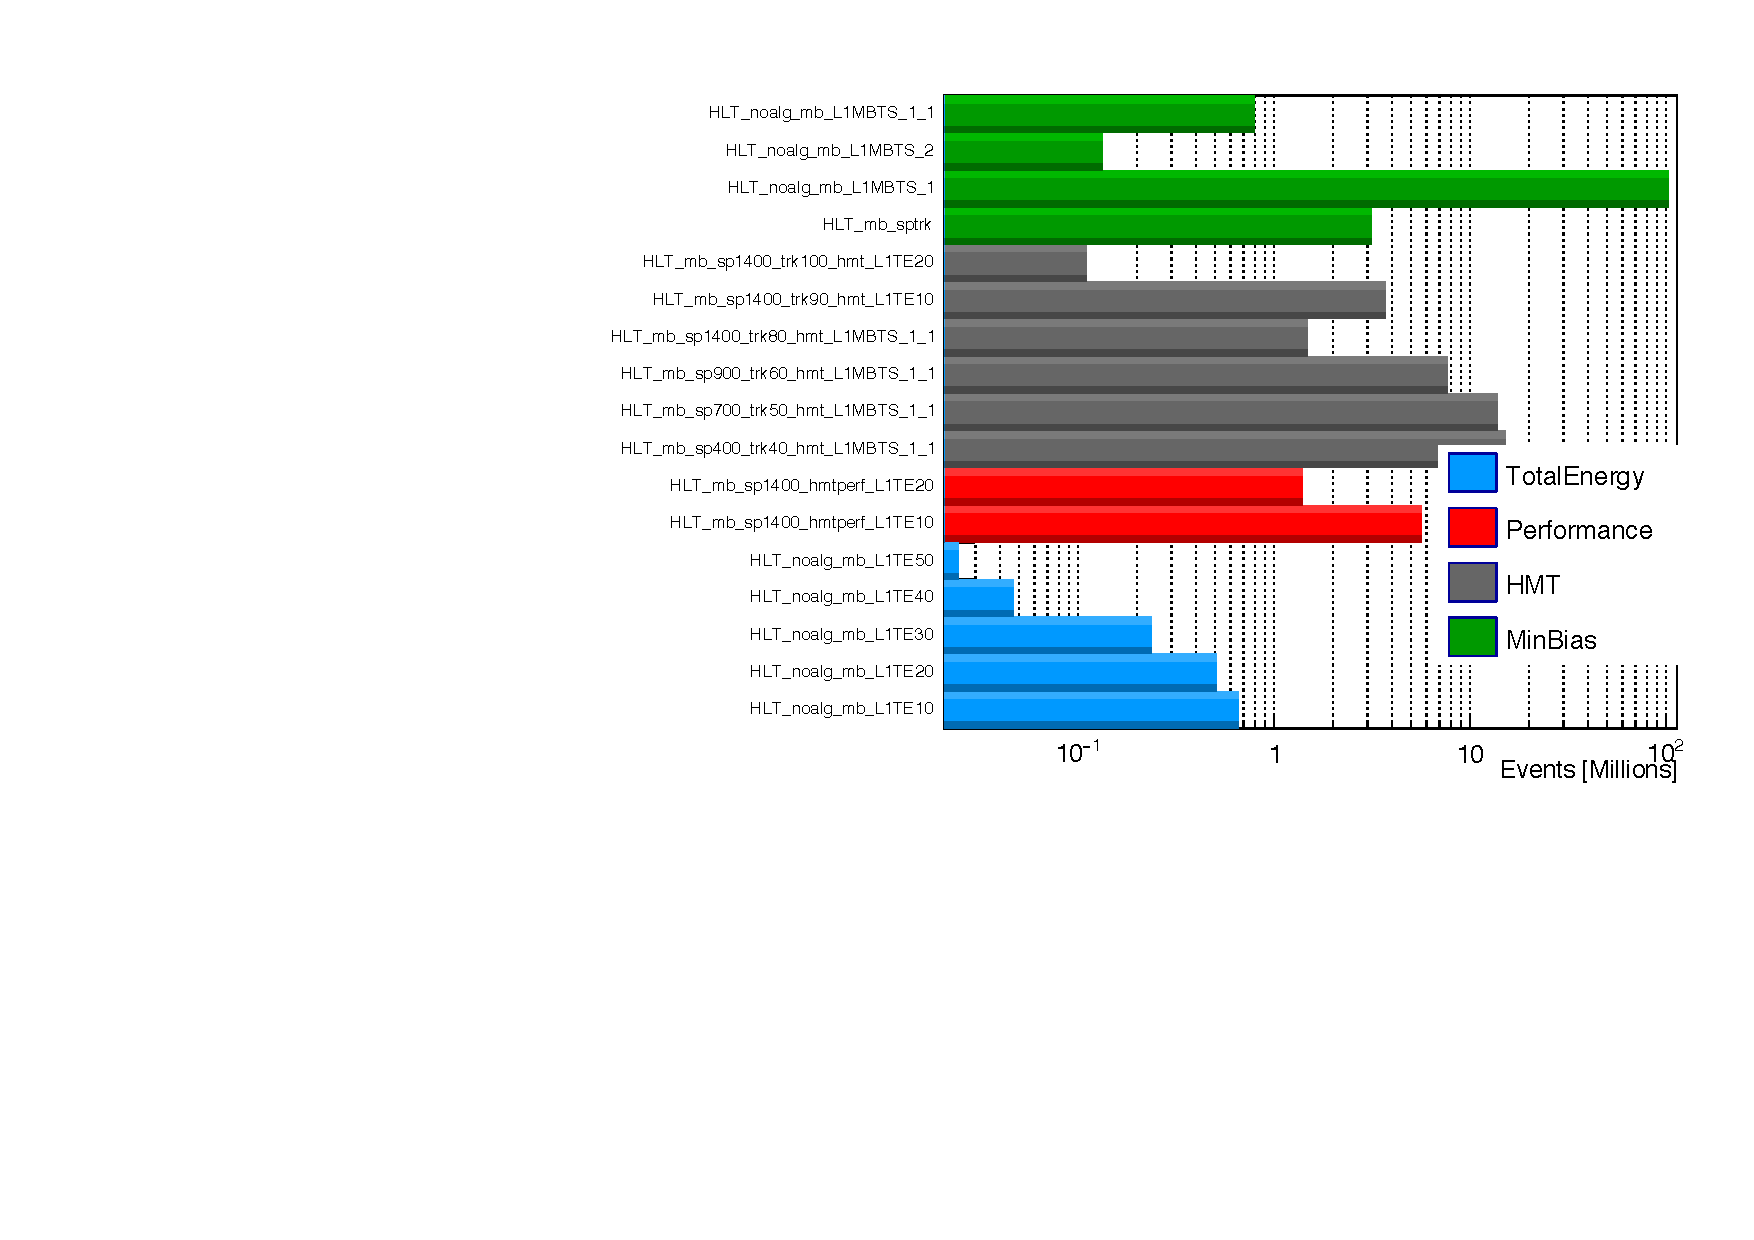
\includegraphics[width=.9\linewidth]{figs/sec_evtSlc/stat_pp13_run1.pdf}
\caption{Total statistics of all the MinBias and HMT related triggers, recorded in 13 TeV $pp$ run period 1.}
\label{fig:stat_pp13_run1}
\end{figure}

\begin{figure}[H]
\centering
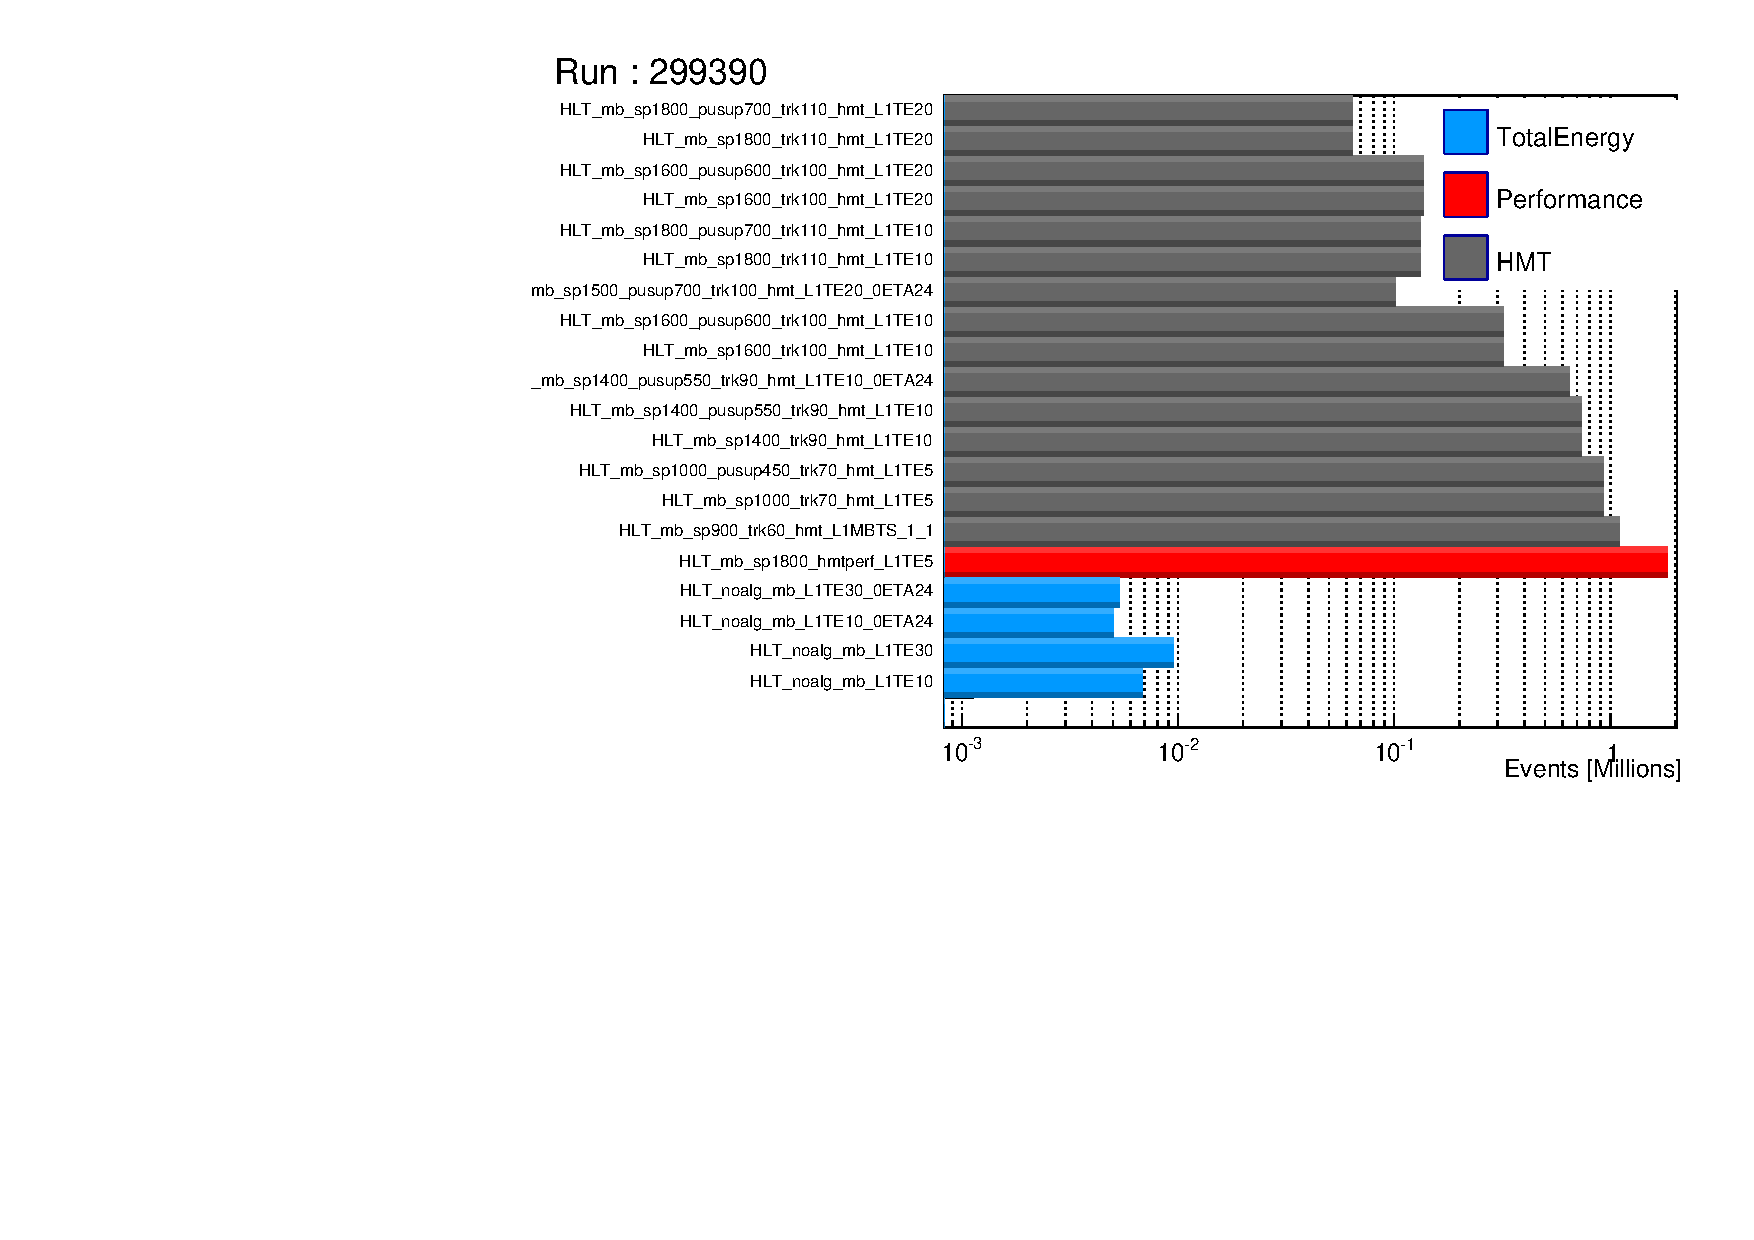
\includegraphics[width=.9\linewidth]{figs/sec_evtSlc/stat_pp13_run2_1.pdf}
\caption{Total statistics of all the MinBias and HMT related triggers, recorded in 13 TeV $pp$ run period 2 (299390).}
\label{fig:stat_pp13_run2}
\end{figure}

\begin{figure}[H]
\centering
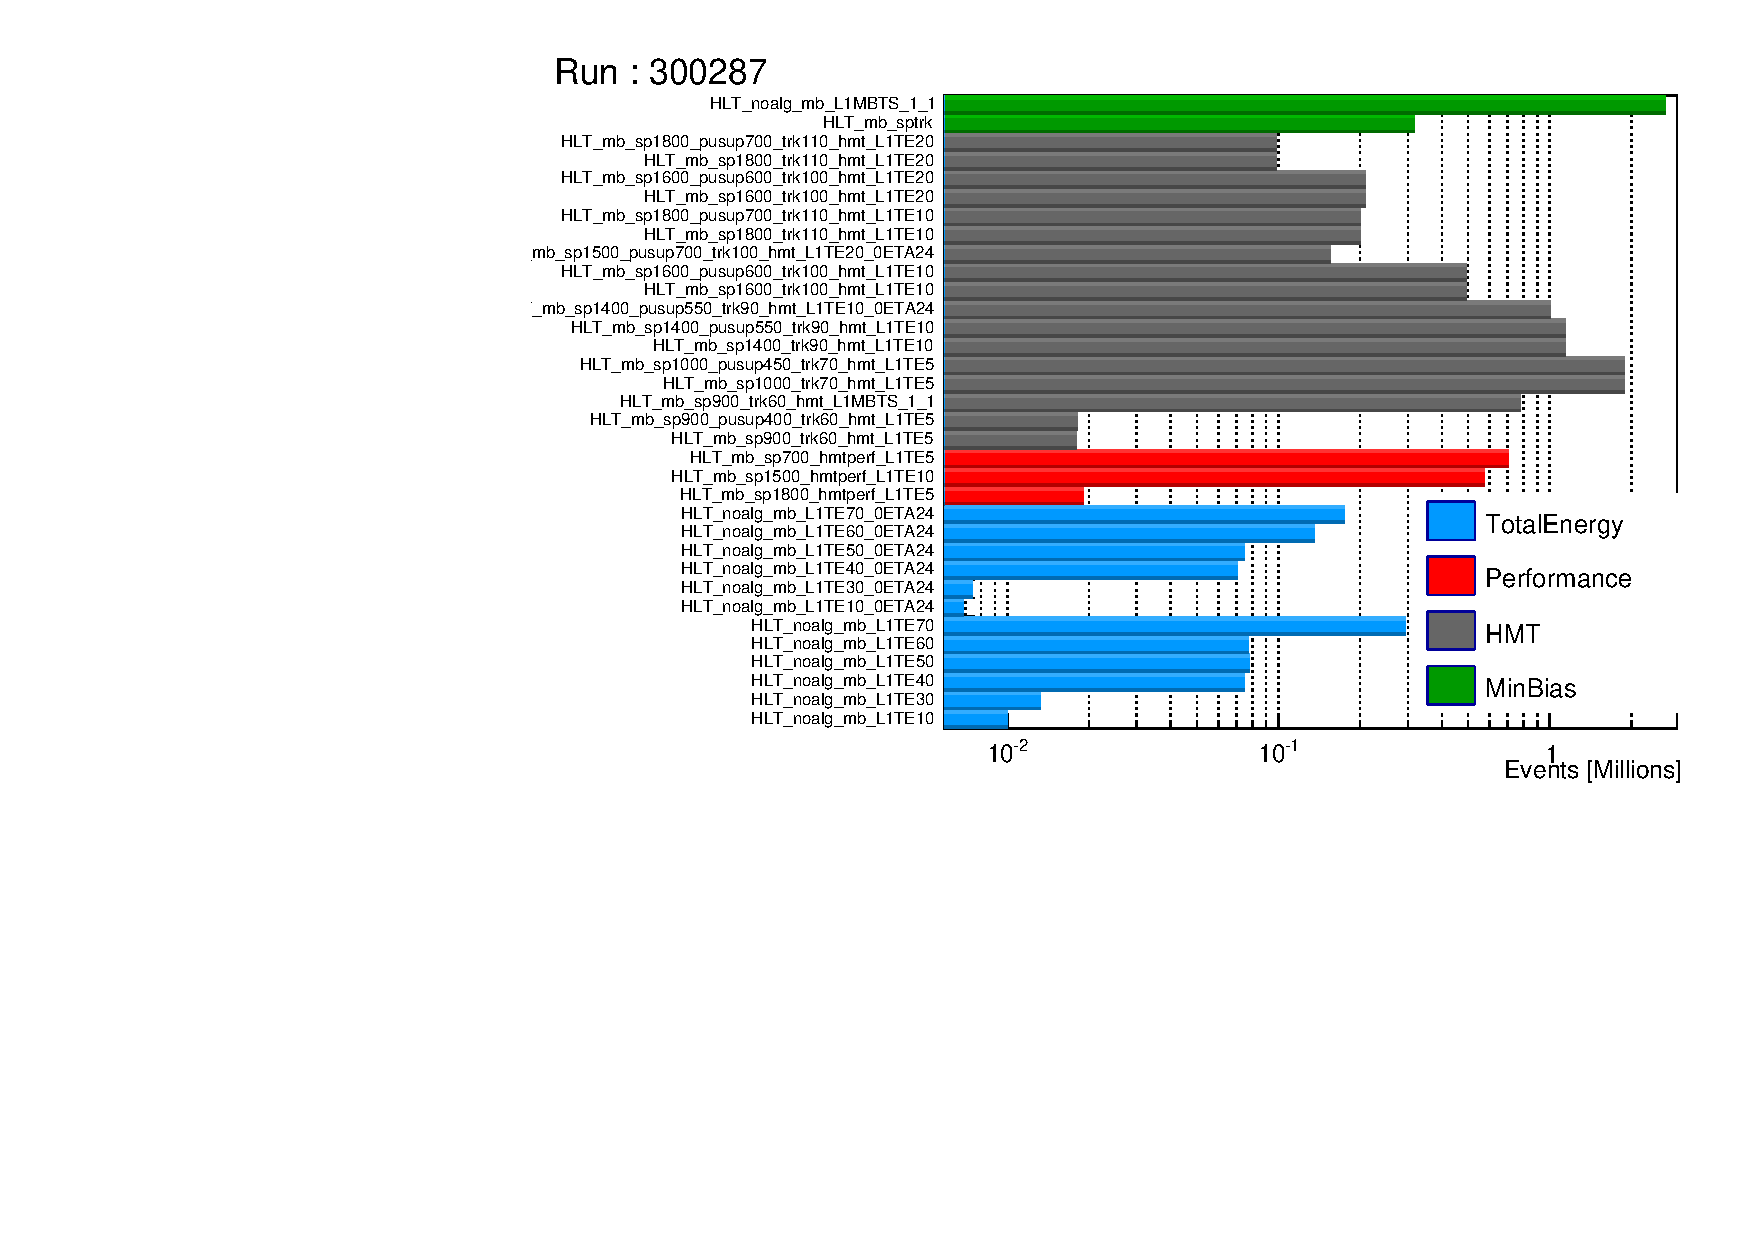
\includegraphics[width=.9\linewidth]{figs/sec_evtSlc/stat_pp13_run2_2.pdf}
\caption{Total statistics of all the MinBias and HMT related triggers, recorded in 13 TeV $pp$ run period 2 (300287).}
\label{fig:stat_pp13_run2}
\end{figure}

\begin{figure}[H]
\centering
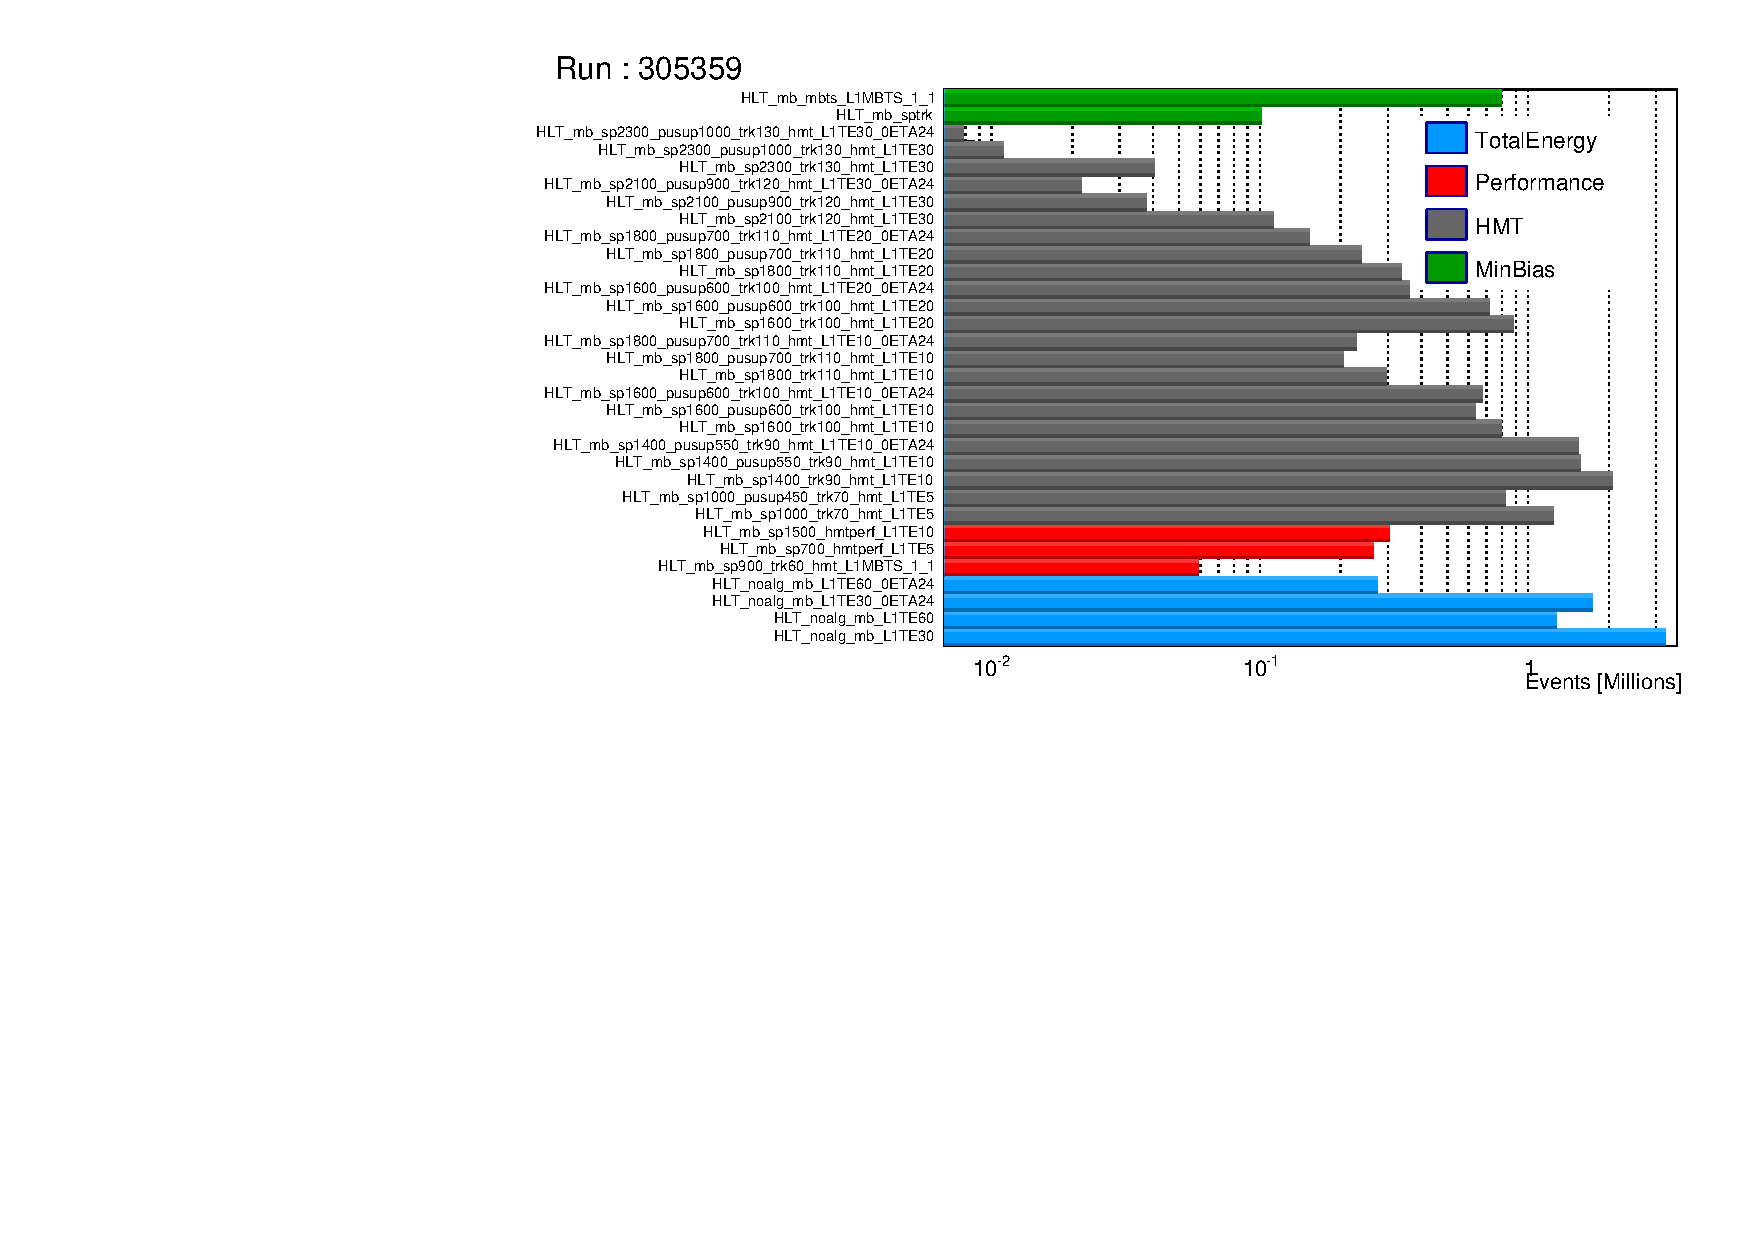
\includegraphics[width=.9\linewidth]{figs/sec_evtSlc/stat_pp13_run3.pdf}
\caption{Total statistics of all the MinBias and HMT related triggers, recorded in 13 TeV $pp$ run period 3.}
\label{fig:stat_pp13_run3}
\end{figure}

\begin{figure}[H]
\centering
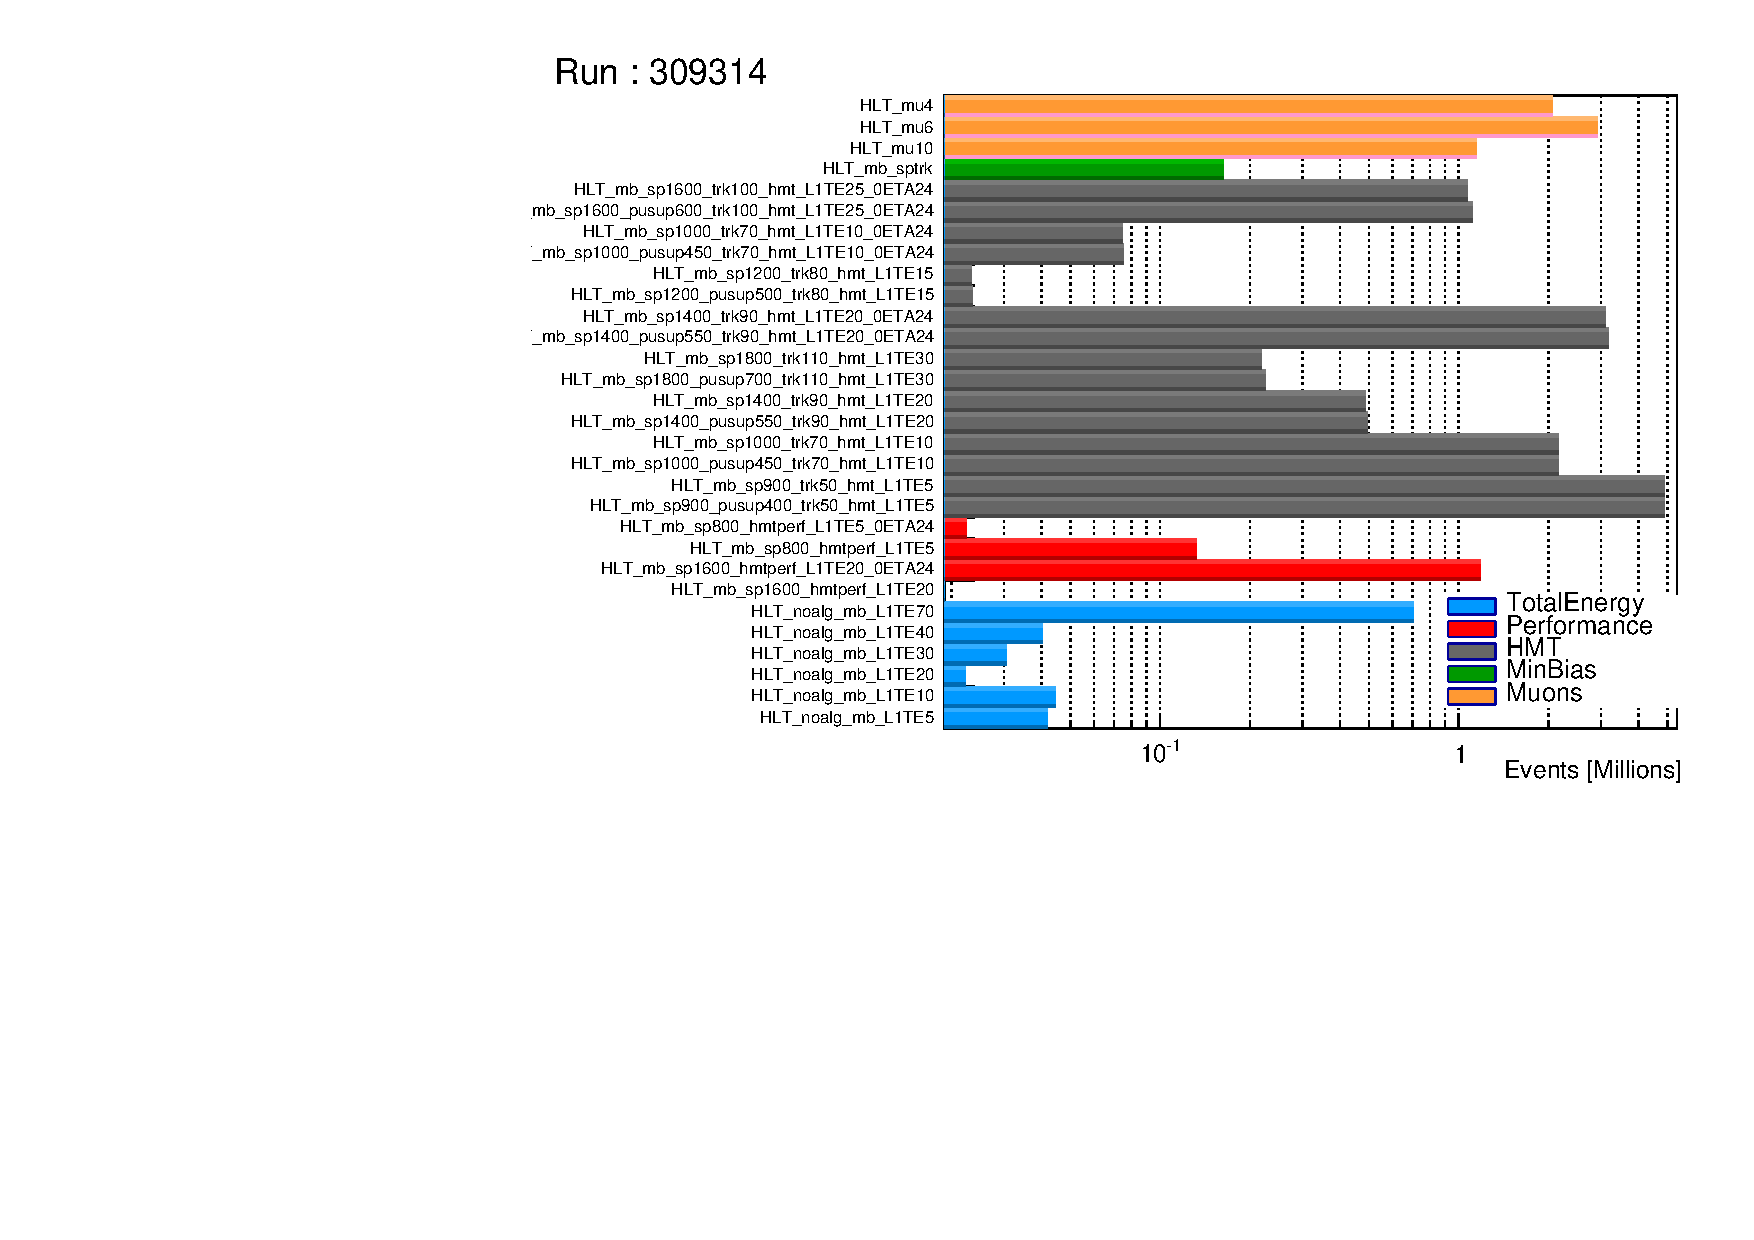
\includegraphics[width=.9\linewidth]{figs/sec_evtSlc/stat_pp13_run4_1.pdf}
\caption{Total statistics of all the MinBias and HMT related triggers, recorded in 13 TeV $pp$ run period 4 (309314).}
\label{fig:stat_pp13_run4}
\end{figure}

\begin{figure}[H]
\centering
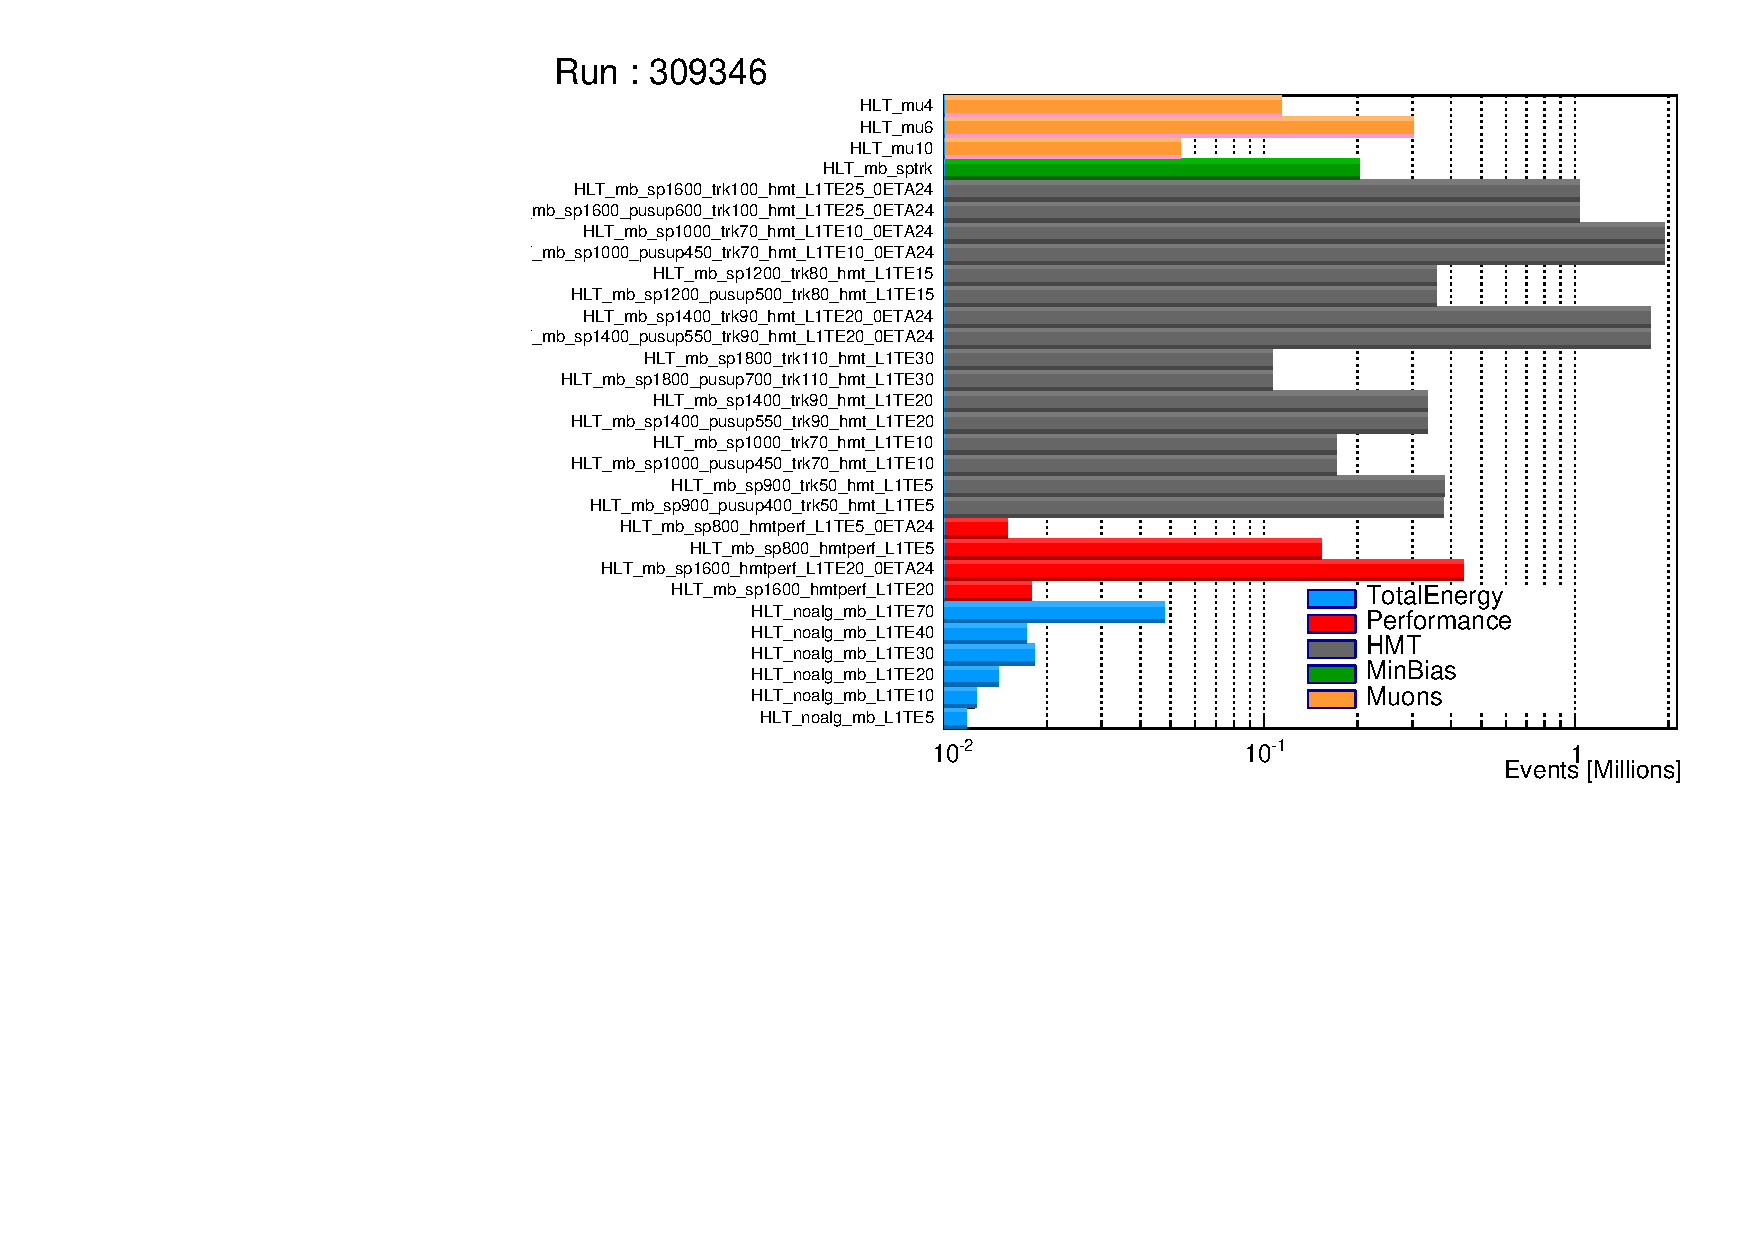
\includegraphics[width=.9\linewidth]{figs/sec_evtSlc/stat_pp13_run4_2.pdf}
\caption{Total statistics of all the MinBias and HMT related triggers, recorded in 13 TeV $pp$ run period 4 (309346).}
\label{fig:stat_pp13_run4}
\end{figure}

\begin{figure}[H]
\centering
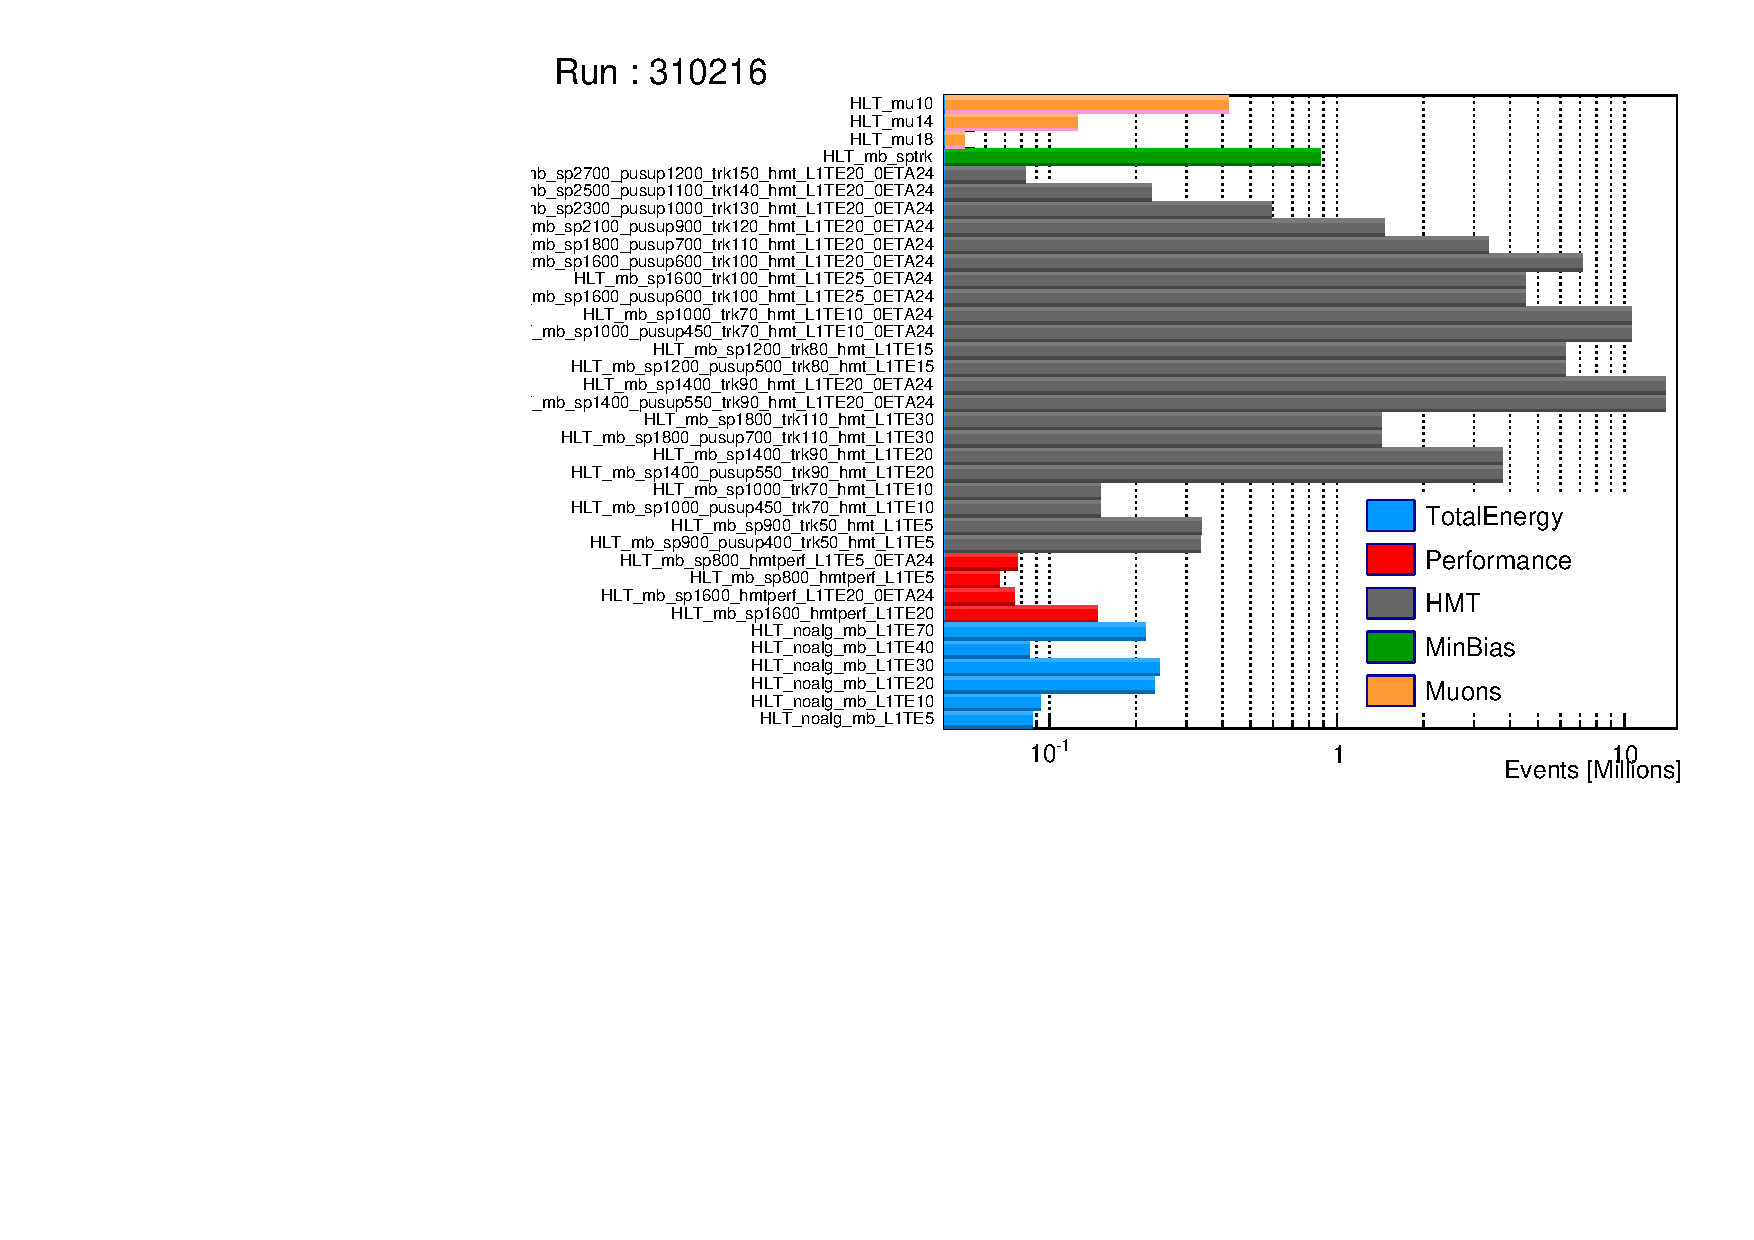
\includegraphics[width=.9\linewidth]{figs/sec_evtSlc/stat_pp13_run4_3.pdf}
\caption{Total statistics of all the MinBias and HMT related triggers, recorded in 13 TeV $pp$ run period 4 (310216).}
\label{fig:stat_pp13_run4}
\end{figure}



\subsection{Statistics of all triggers in $pp$ 5.02 TeV}
\begin{figure}[H]
\centering
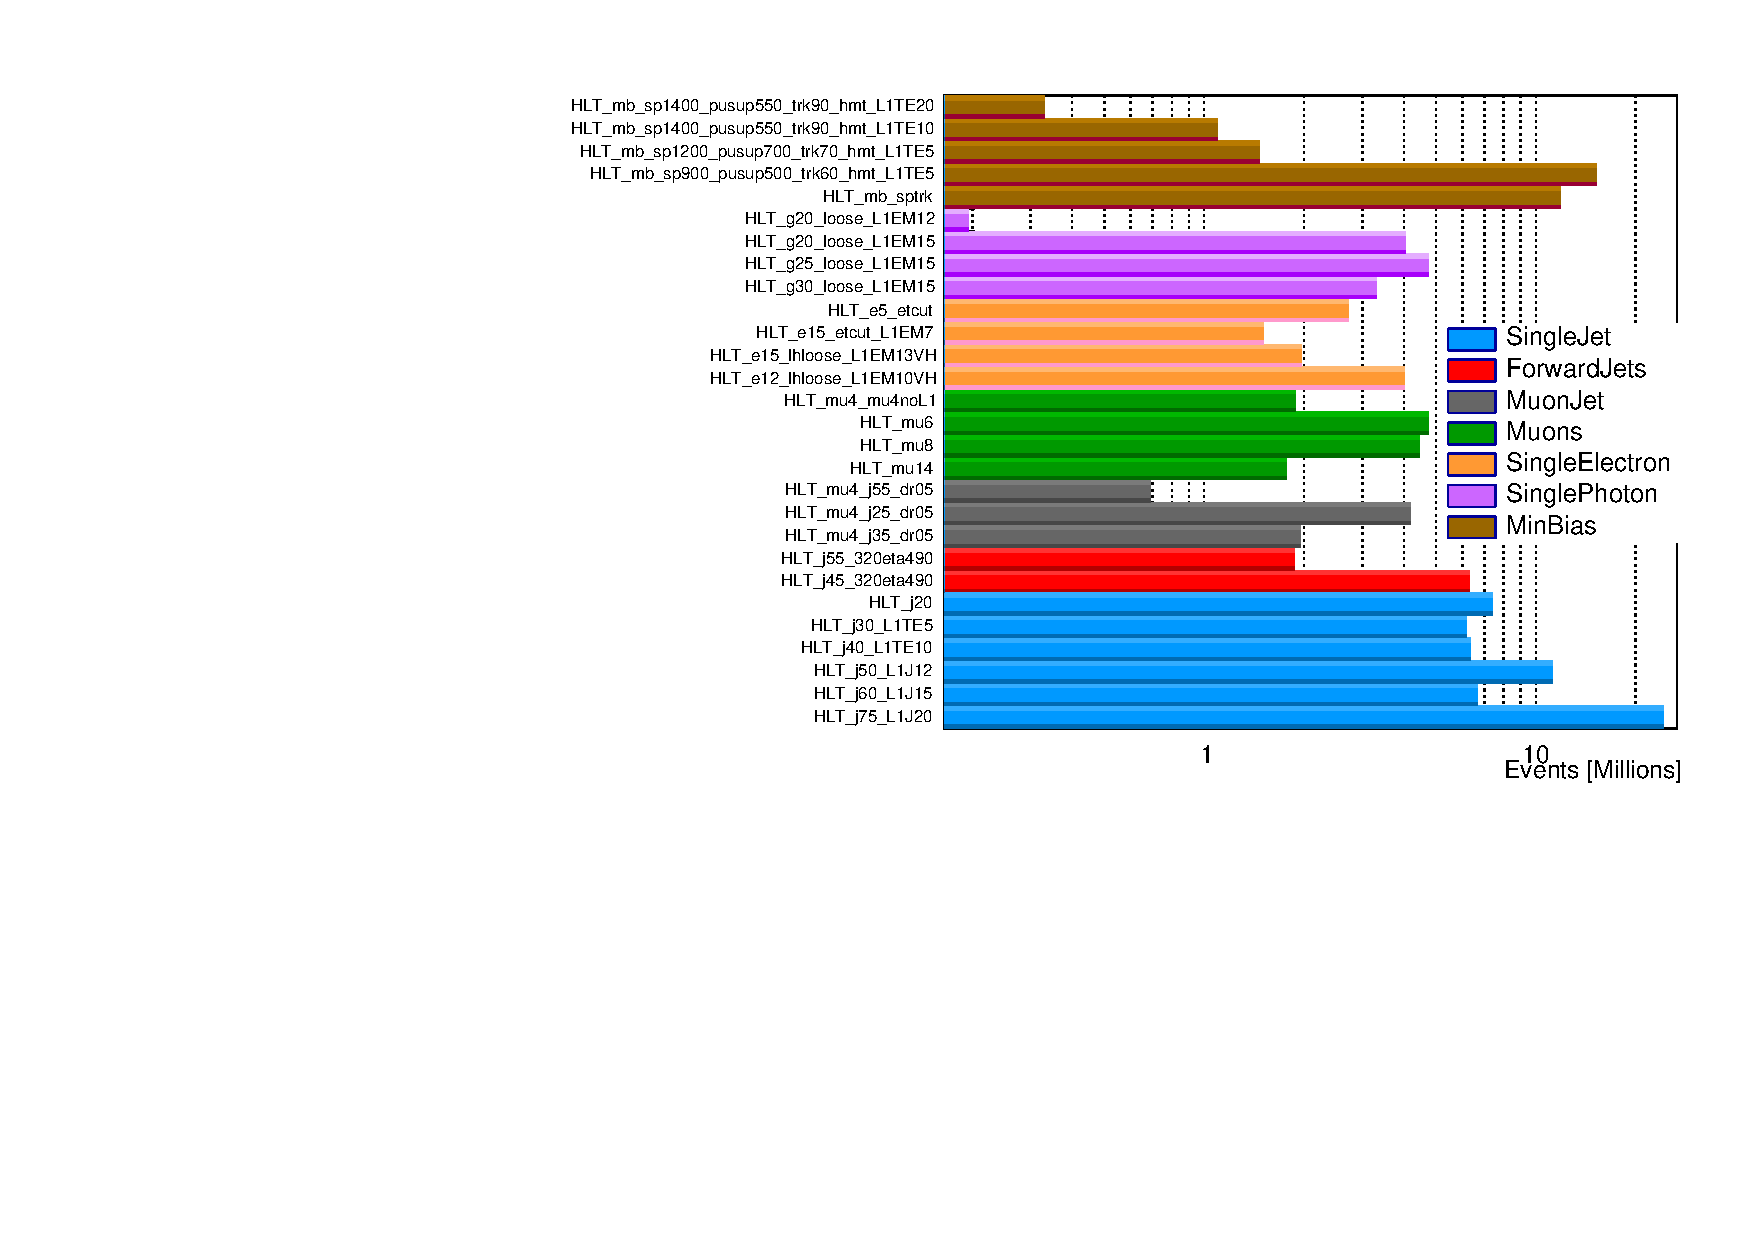
\includegraphics[width=.9\linewidth]{figs/sec_evtSlc/stat_pp5.pdf}
\caption{Total statistics of all the MinBias and HMT related triggers, recorded in 5 TeV $pp$ reference run.}
\label{fig:stat_pp5}
\end{figure}



\subsection{Auxiliary plots 13 TeV PYTHIA}
Fig.~\ref{fig:trkEff_pp13_mon_evt} shows the performance of event-level quantities in this PYTHIA sample, both for truth and reconstructed. For the $z$ position, the mean value is shifted by -10$mm$ and the distribution is roughly Gaussian. The correlation between $z$ positions of truth and reconstructed vertex are very strong. The number of charged particles is determined by counting number of tracking passing the tracking selection criteria, which will be introduced later. The 3 bumps shown in the distribution represents the 3 million high-multiplicity events. The number of reconstructed tracks is smaller than truth due to the efficiency loss. The correlation between the number of truth and reconstructed tracks is also strong, as shown in the right plot.

\begin{figure}[H]

\begin{subfigure}{0.5\textwidth}
\centering
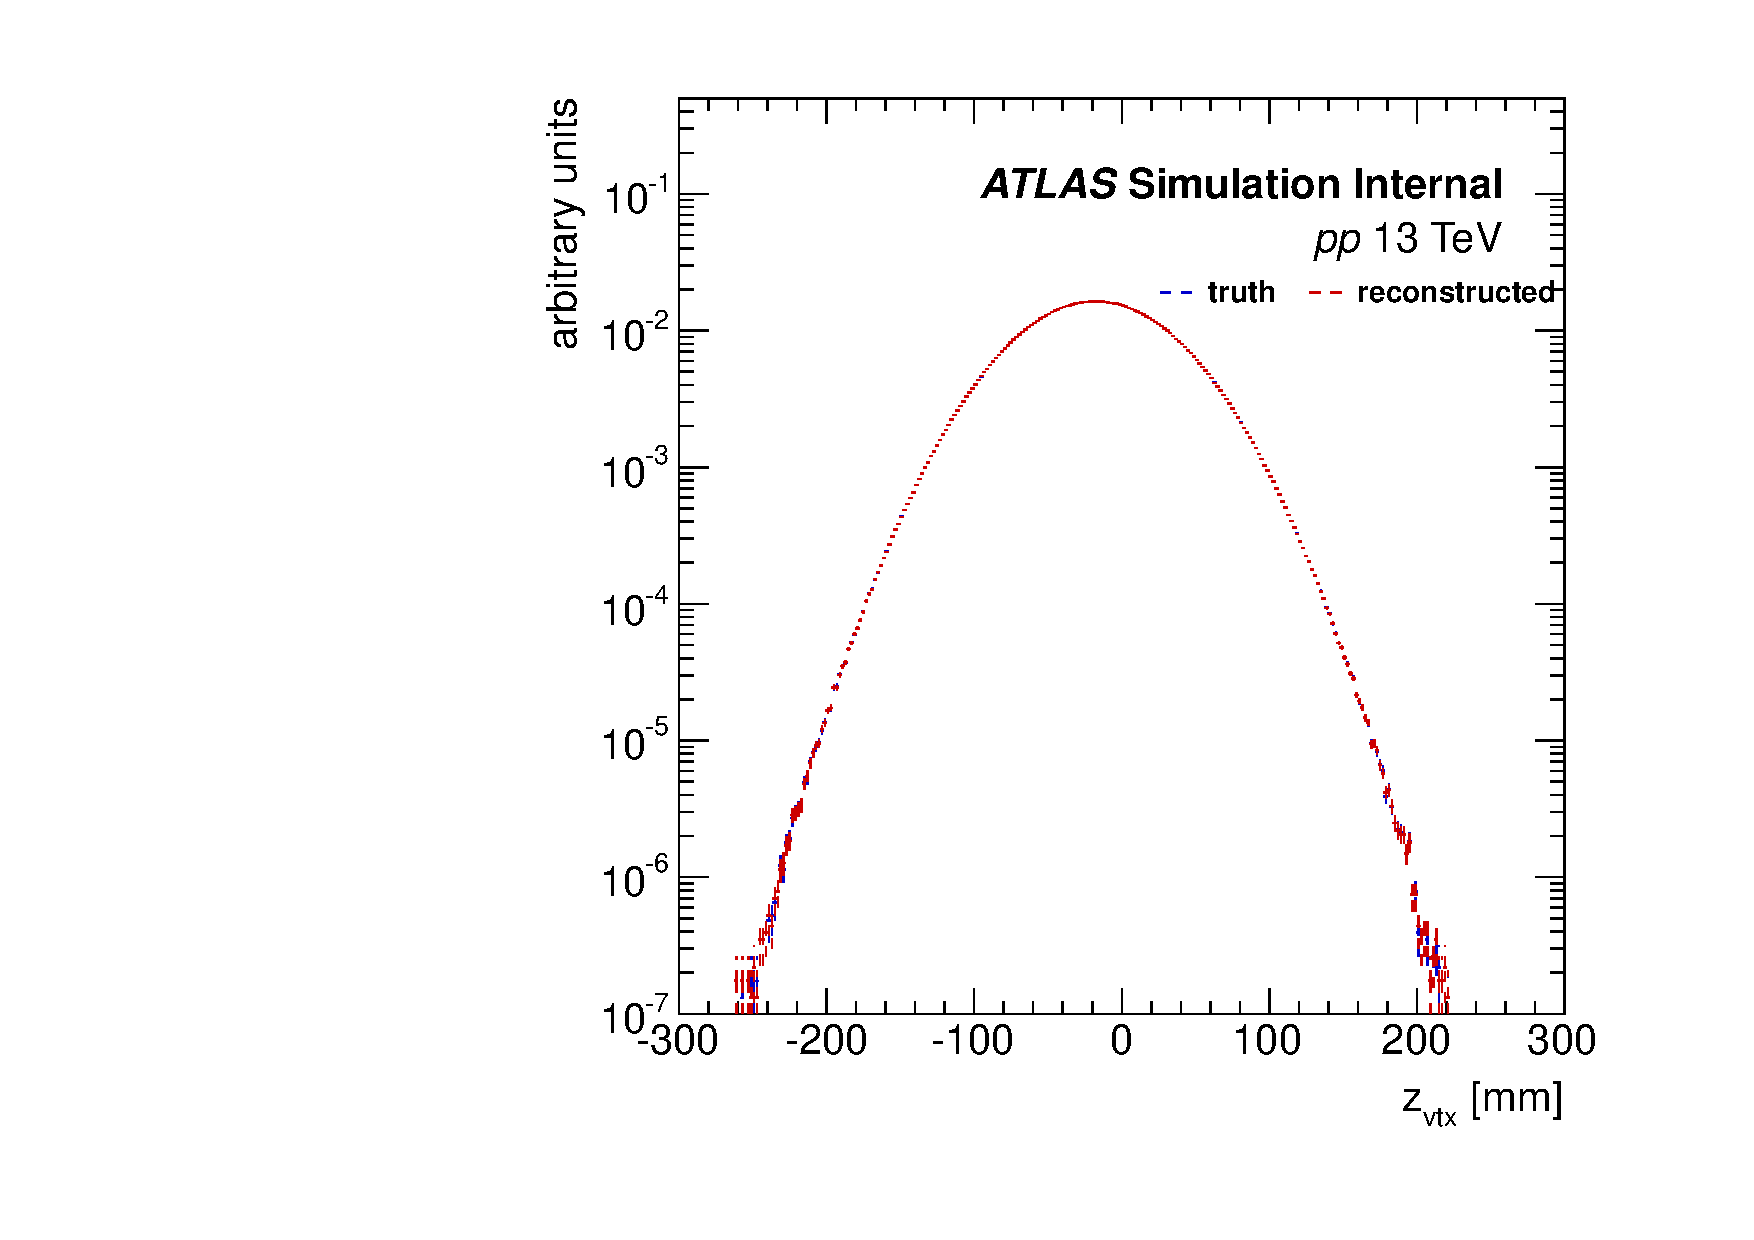
\includegraphics[width=1.\linewidth]{figs/sec_evtSlc/trkEff_pp13_mon_dis_zVtx.pdf}
\caption{Distribution of $z$ position.}
\end{subfigure}
\begin{subfigure}{0.5\textwidth}
\centering
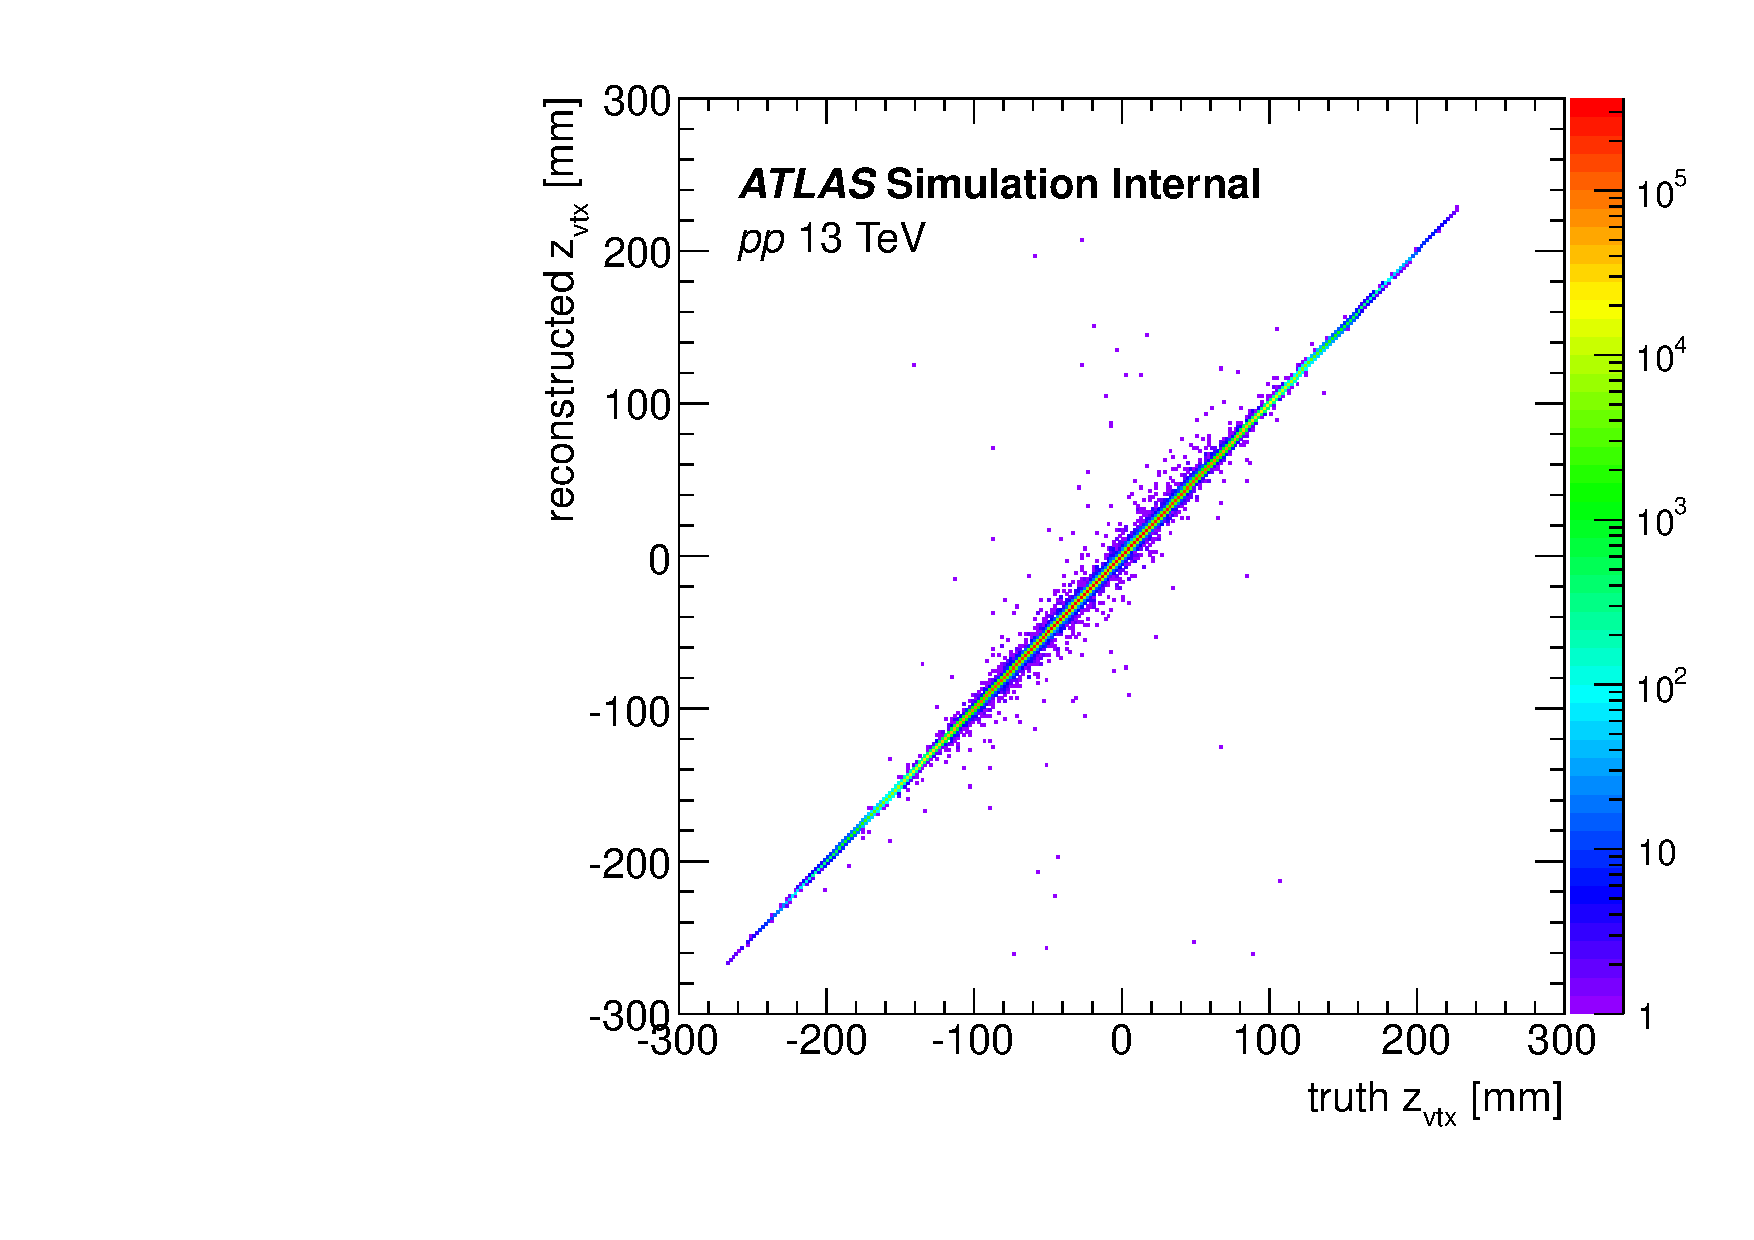
\includegraphics[width=1.\linewidth]{figs/sec_evtSlc/trkEff_pp13_mon_crr_zVtx.pdf}
\caption{Correlation of truth and reconstructed.}
\end{subfigure}
\begin{subfigure}{0.5\textwidth}
\centering
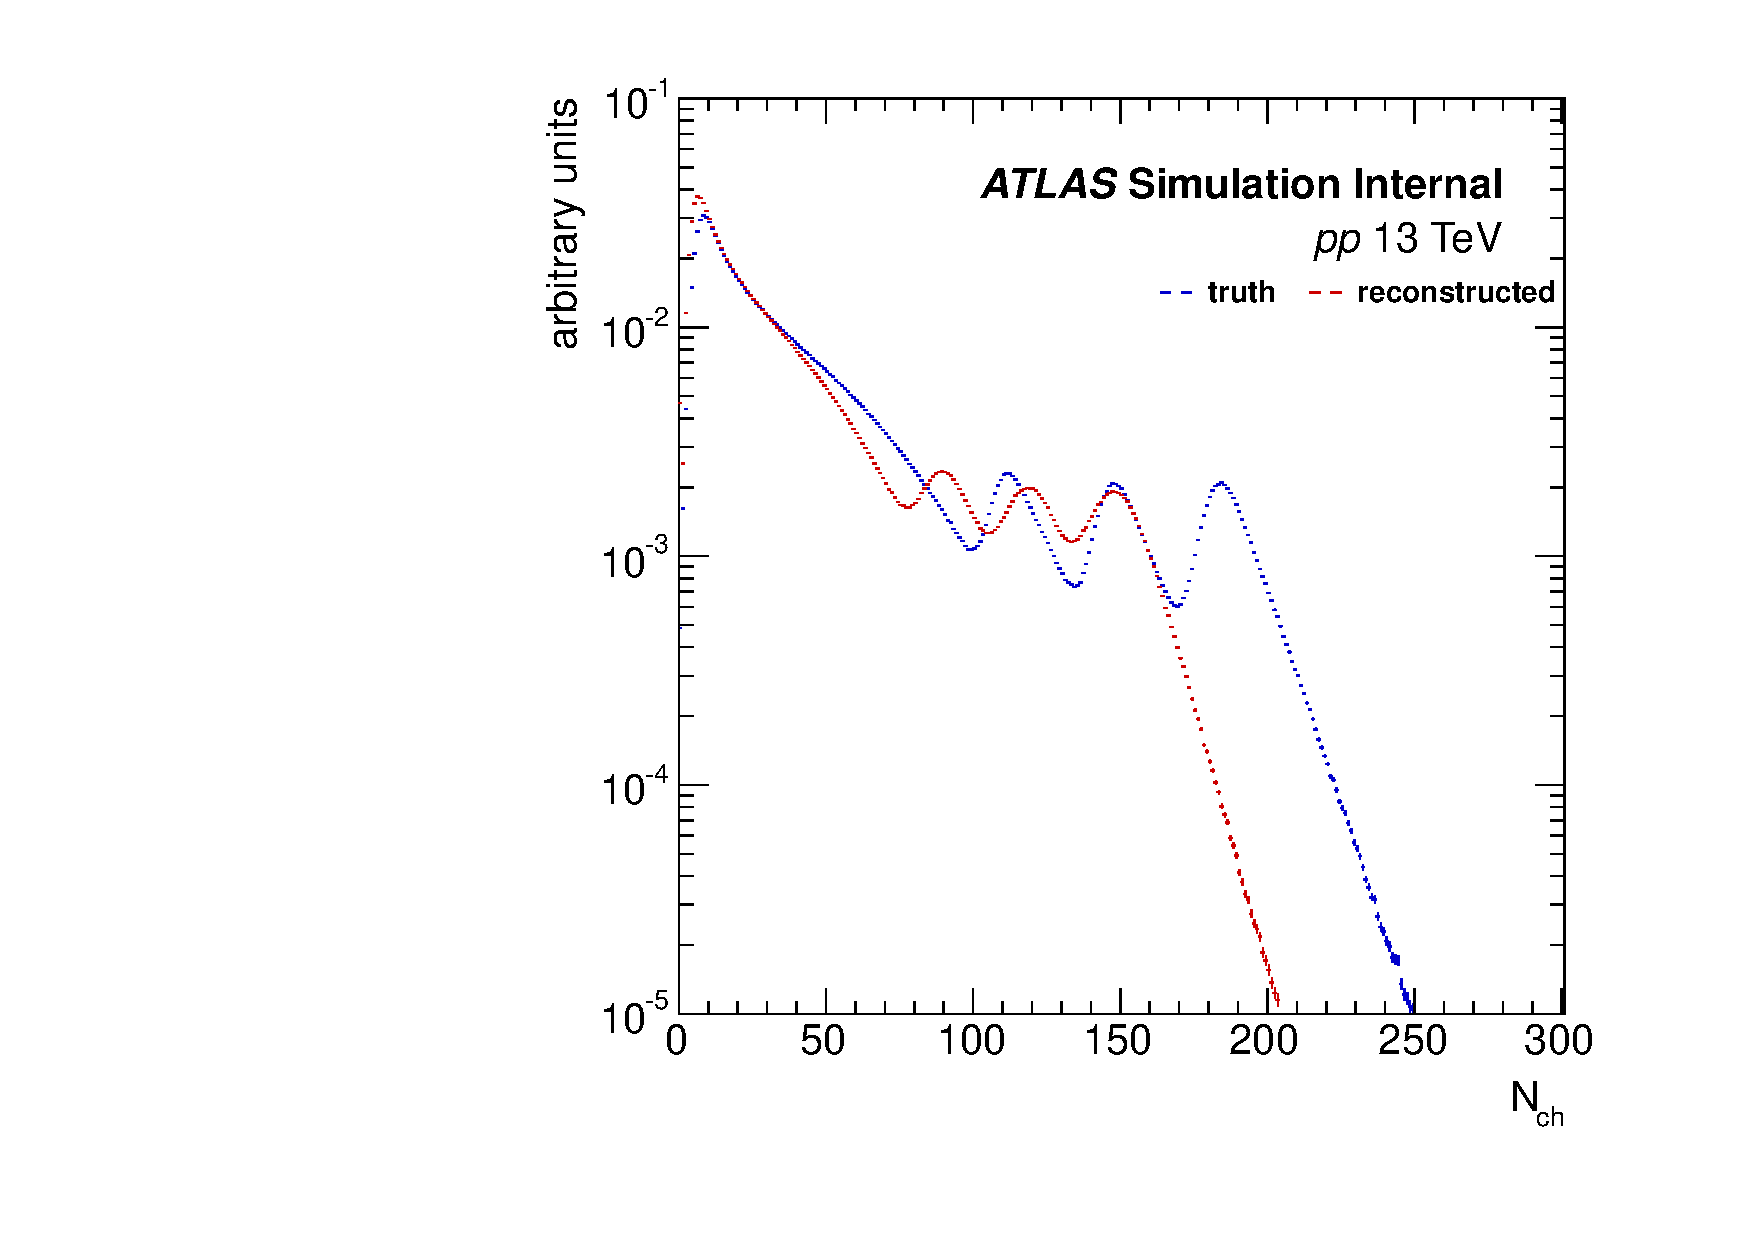
\includegraphics[width=1.\linewidth]{figs/sec_evtSlc/trkEff_pp13_mon_dis_nCh.pdf}
\caption{Distribution of number of charged particles.}
\end{subfigure}
\begin{subfigure}{0.5\textwidth}
\centering
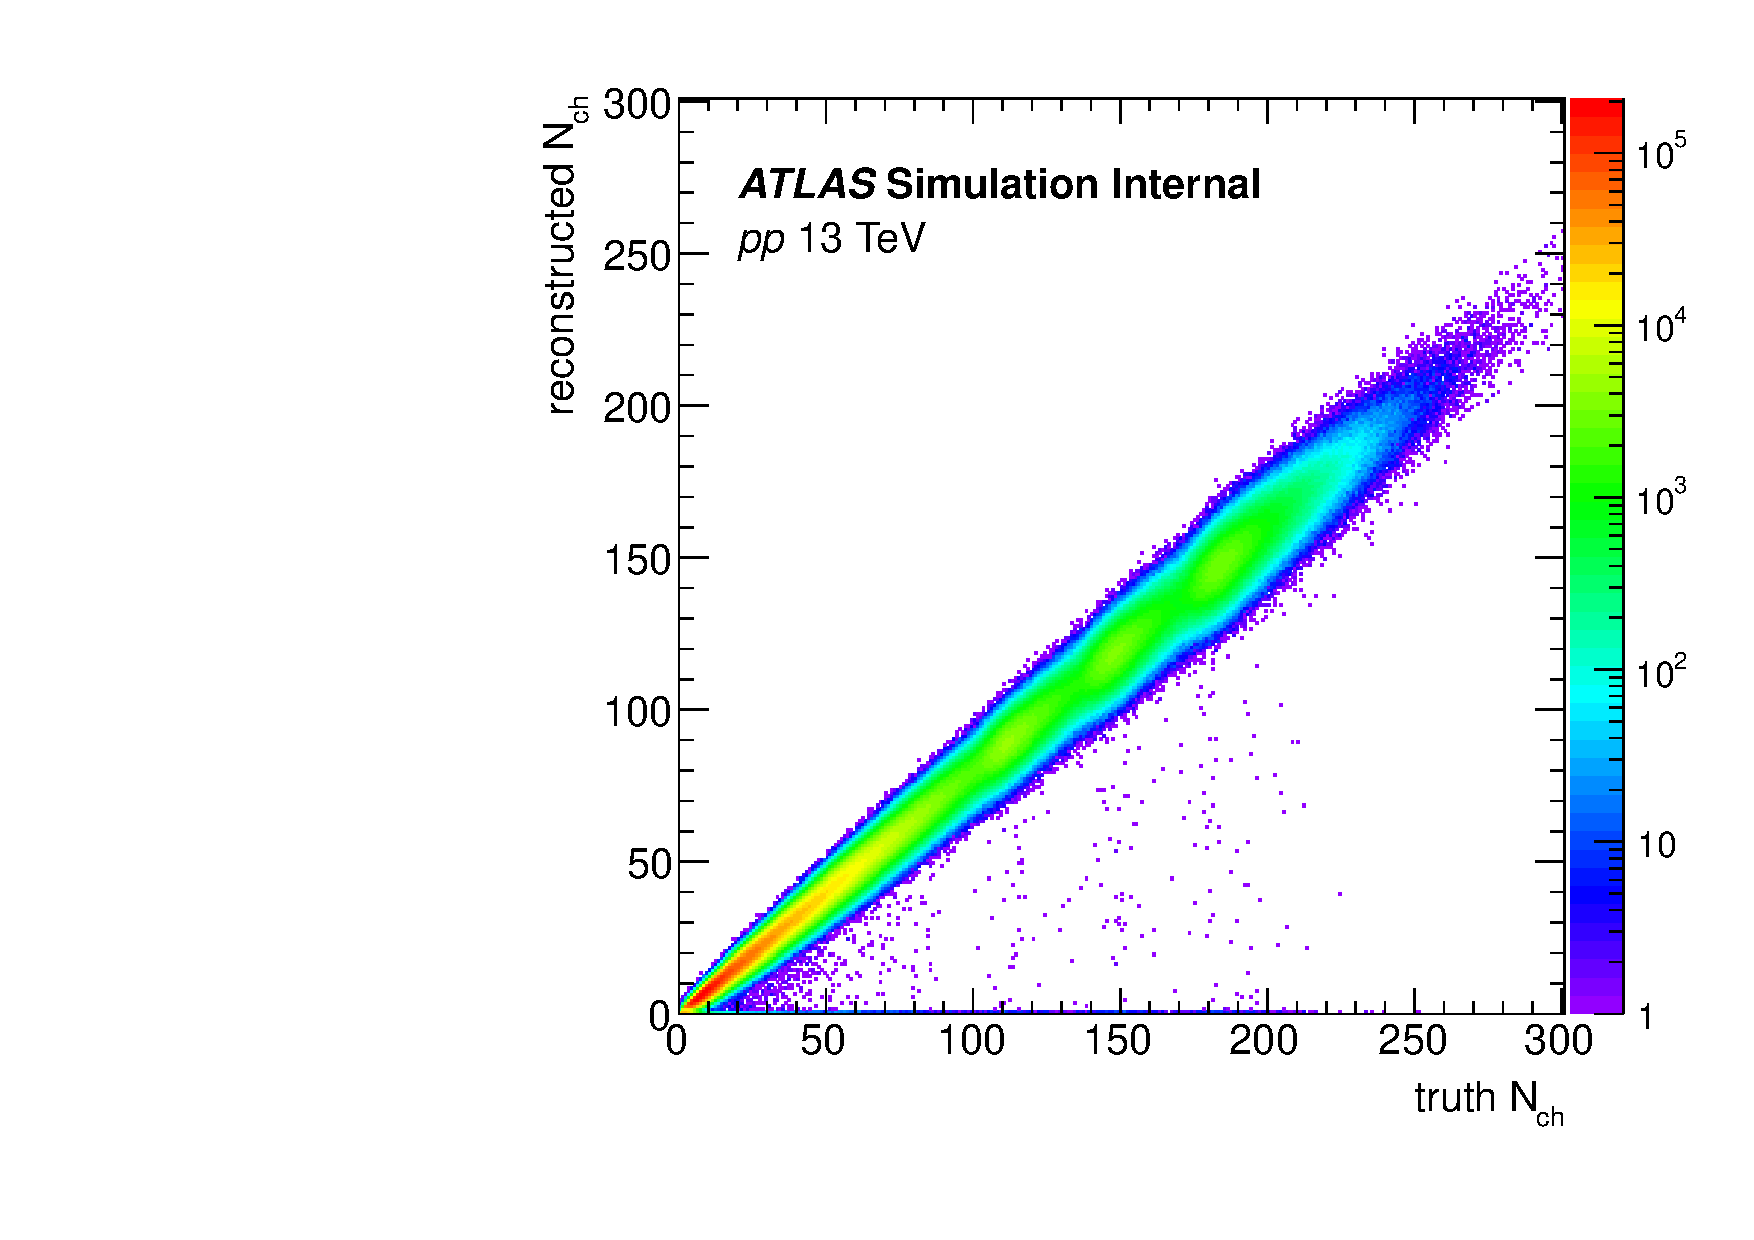
\includegraphics[width=1.\linewidth]{figs/sec_evtSlc/trkEff_pp13_mon_crr_nCh.pdf}
\caption{Correlation of truth and reconstructed.}
\end{subfigure}

\caption{Performance of event-level quantities in PYTHIA 13 TeV $pp$.}
\label{fig:trkEff_pp13_mon_evt}
\end{figure}


The results of particle-level qualities are summarized in Fig.~\ref{fig:trkEff_pp13_mon_trk}, where we compared the three basic quantities of tracking: $p_{T}$, $\eta$ and $\phi$. The $p_{T}$ spectrum is very consistent between truth and reconstructed, while the correlation shows some broad structure in the low-$p_{T}$ region. The distributions of $\eta$ are very different between truth and reconstructed, due to the different efficiency in different $\eta$ region. In this analysis, we will evaluate and apply the tracking efficiency as a function of $\eta$. Based on the correlation plot, the reconstructed and associated truth tracks have consistent $\eta$ value.  For $\phi$ of the charged particles, the reconstructed has additional small structures over truth. We will not apply this efficiency correction in the analysis, instead, we will apply flattening procedure run-by-run. The truth and reconstructed $phi$ are strongly correlated: the events seen in the two corners are due to the periodic boundary condition.

\begin{figure}[H]
\centering
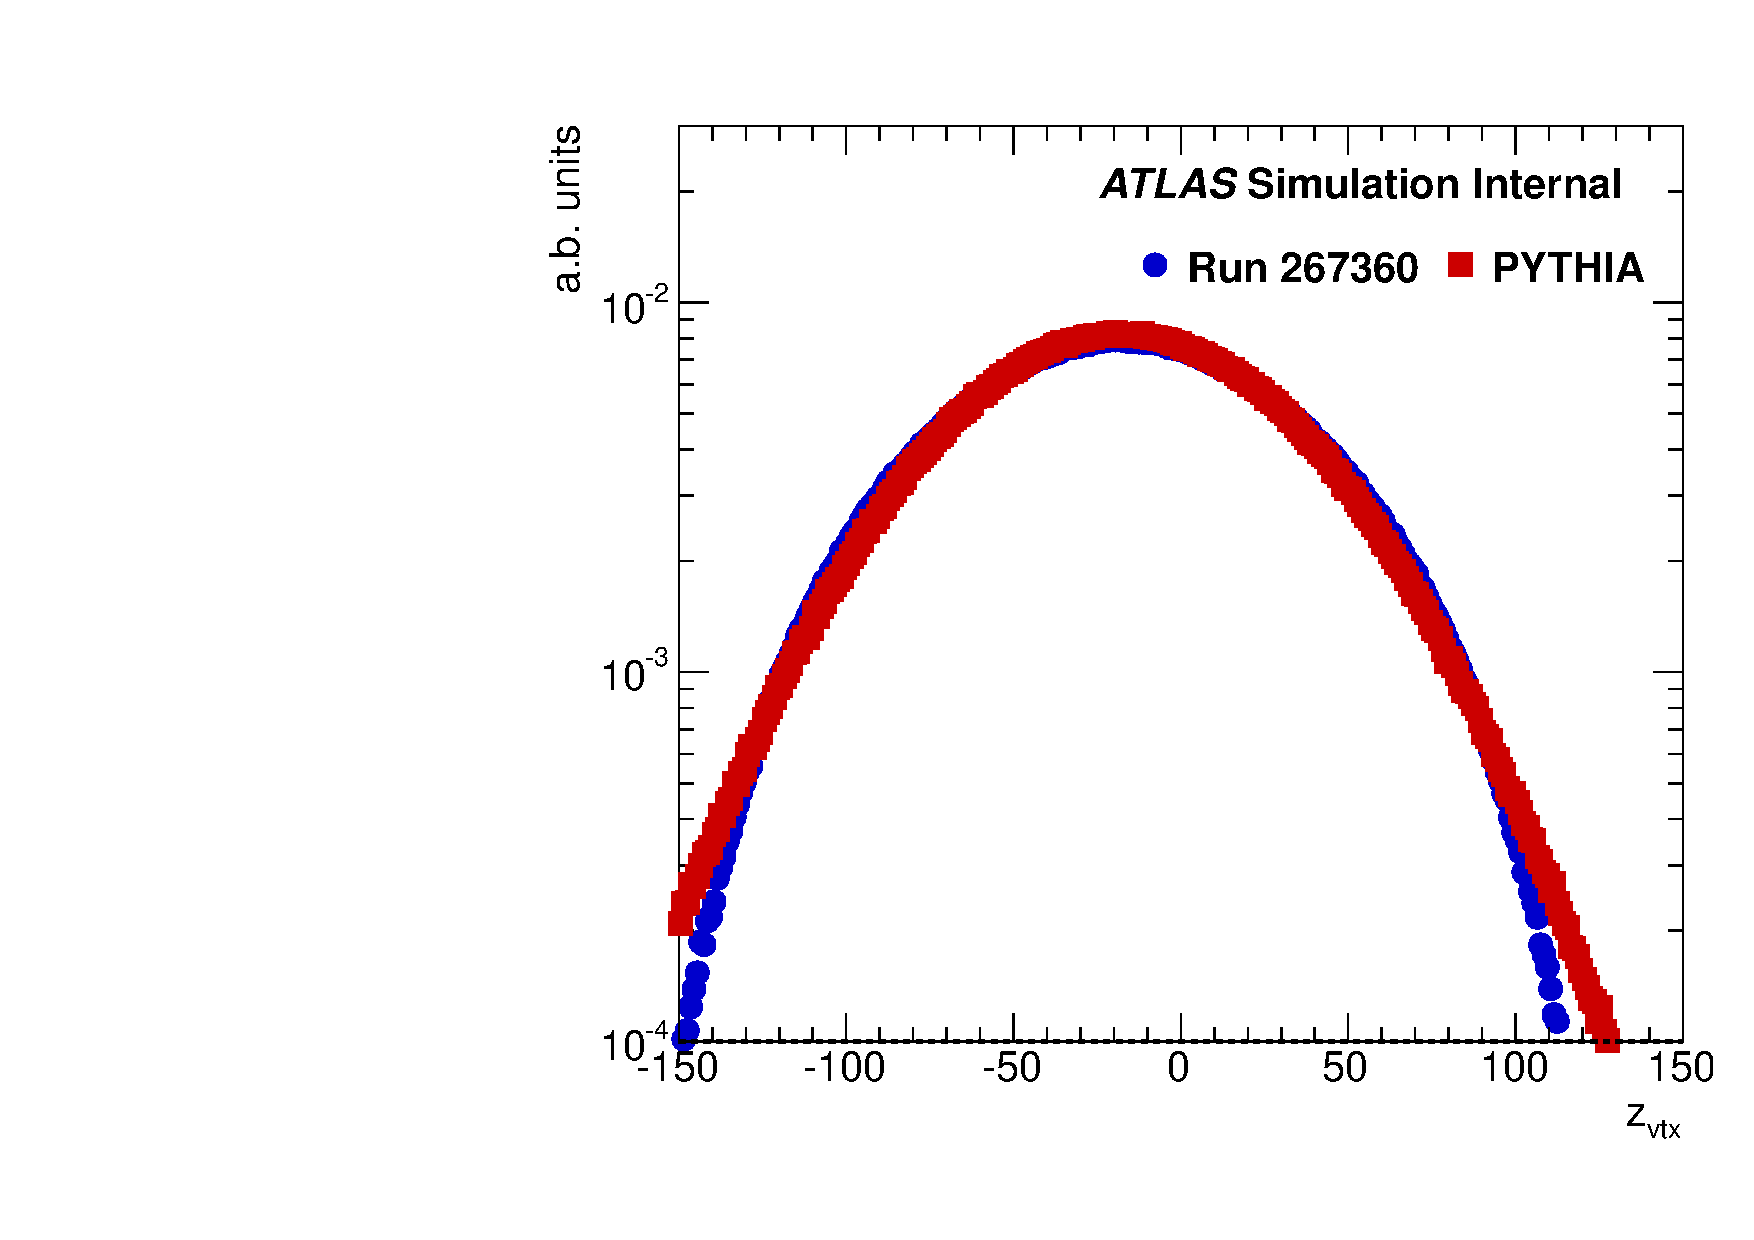
\includegraphics[width=.4\linewidth]{figs/sec_evtSlc/zVtx_MC_data.pdf}
\caption{The distributions of $z_{vertex}$, from Run 267360 and PYTHIA.}
\label{fig:zVtx_MC_data}
\end{figure}
The distribution of $z_{vertex}$ is compared between Run 267360 and PYTHIA, as shown in Fig.~\ref{fig:zVtx_MC_data}. The width of $z_{vertex}$ distribution in PYTHIA is slightly larger than data.

\begin{figure}[H]

\begin{subfigure}{0.5\textwidth}
\centering
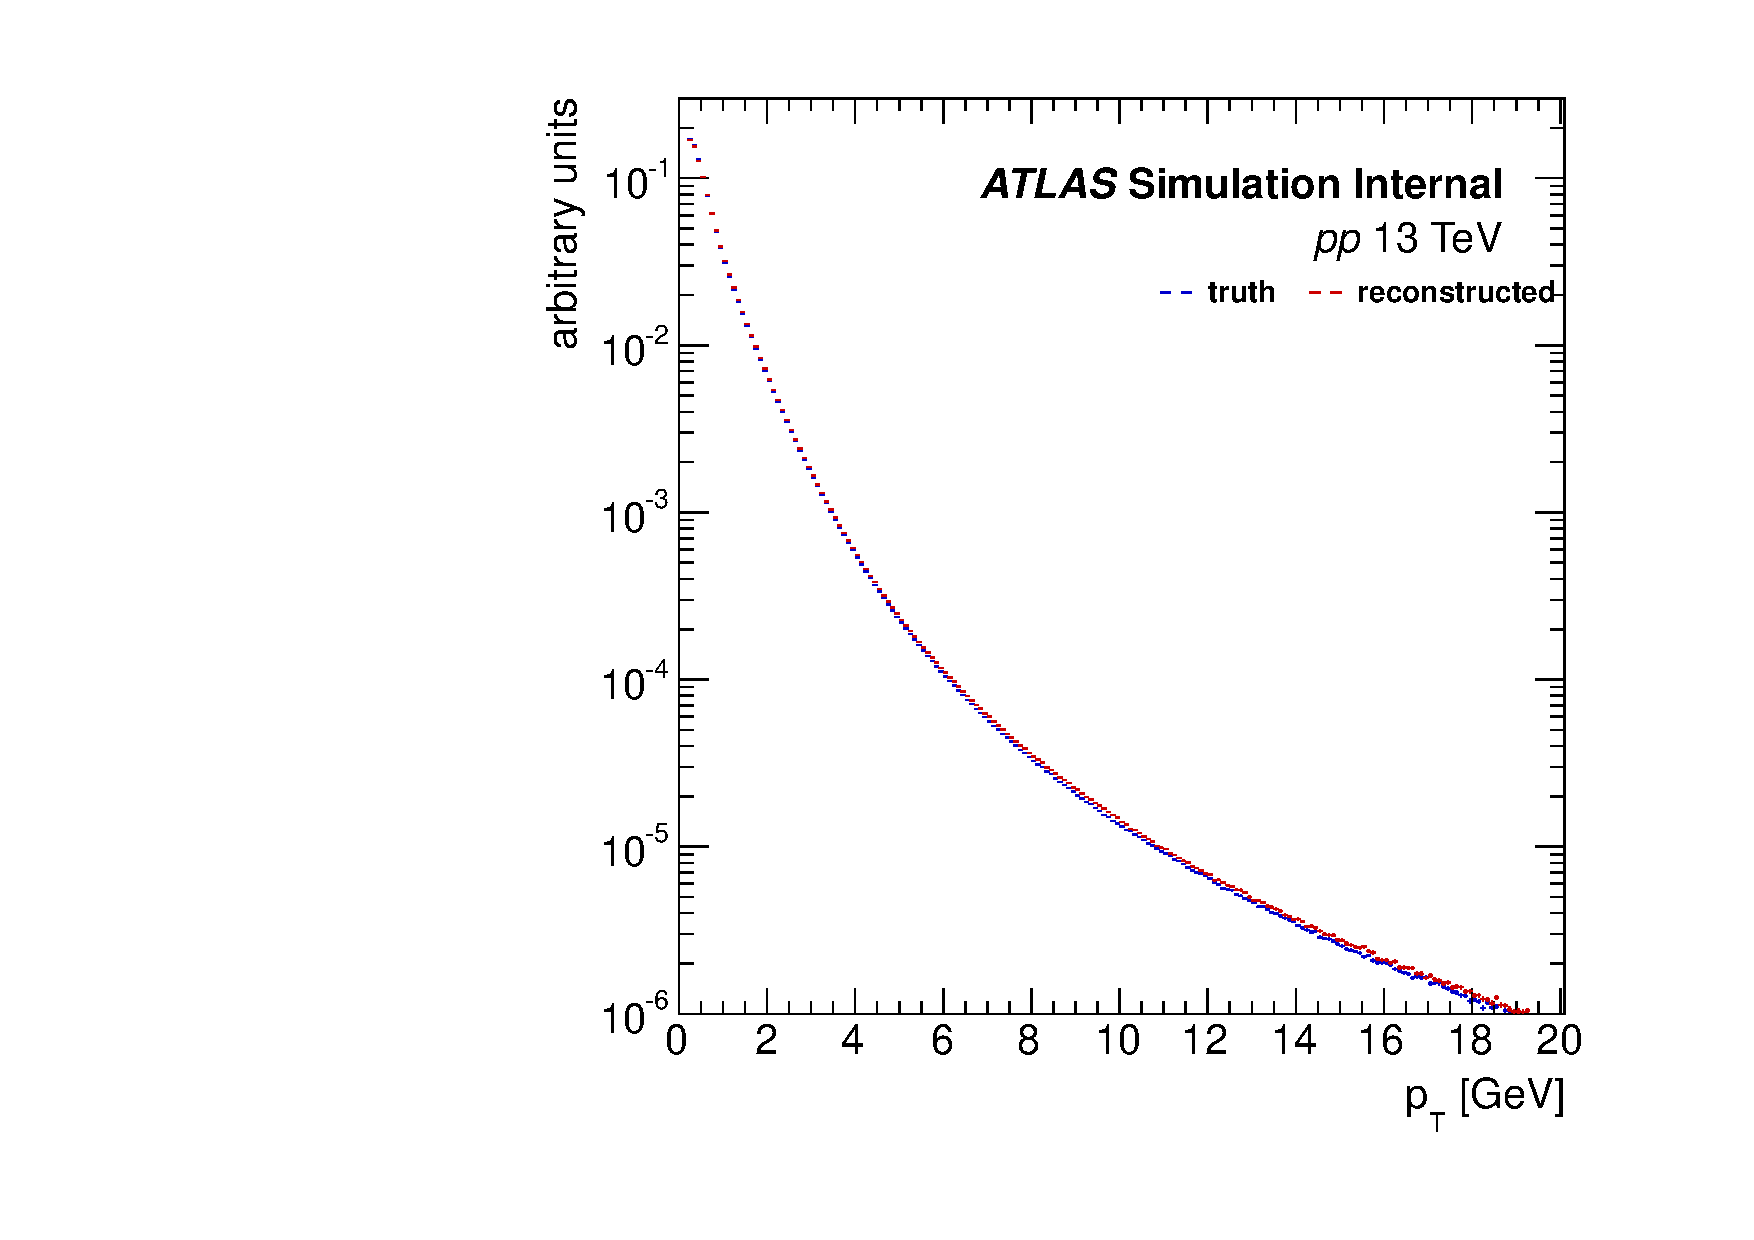
\includegraphics[width=1.\linewidth]{figs/sec_evtSlc/trkEff_pp13_mon_dis_pT.pdf}
\caption{$p_{T}$ spectrum.}
\end{subfigure}
\begin{subfigure}{0.5\textwidth}
\centering
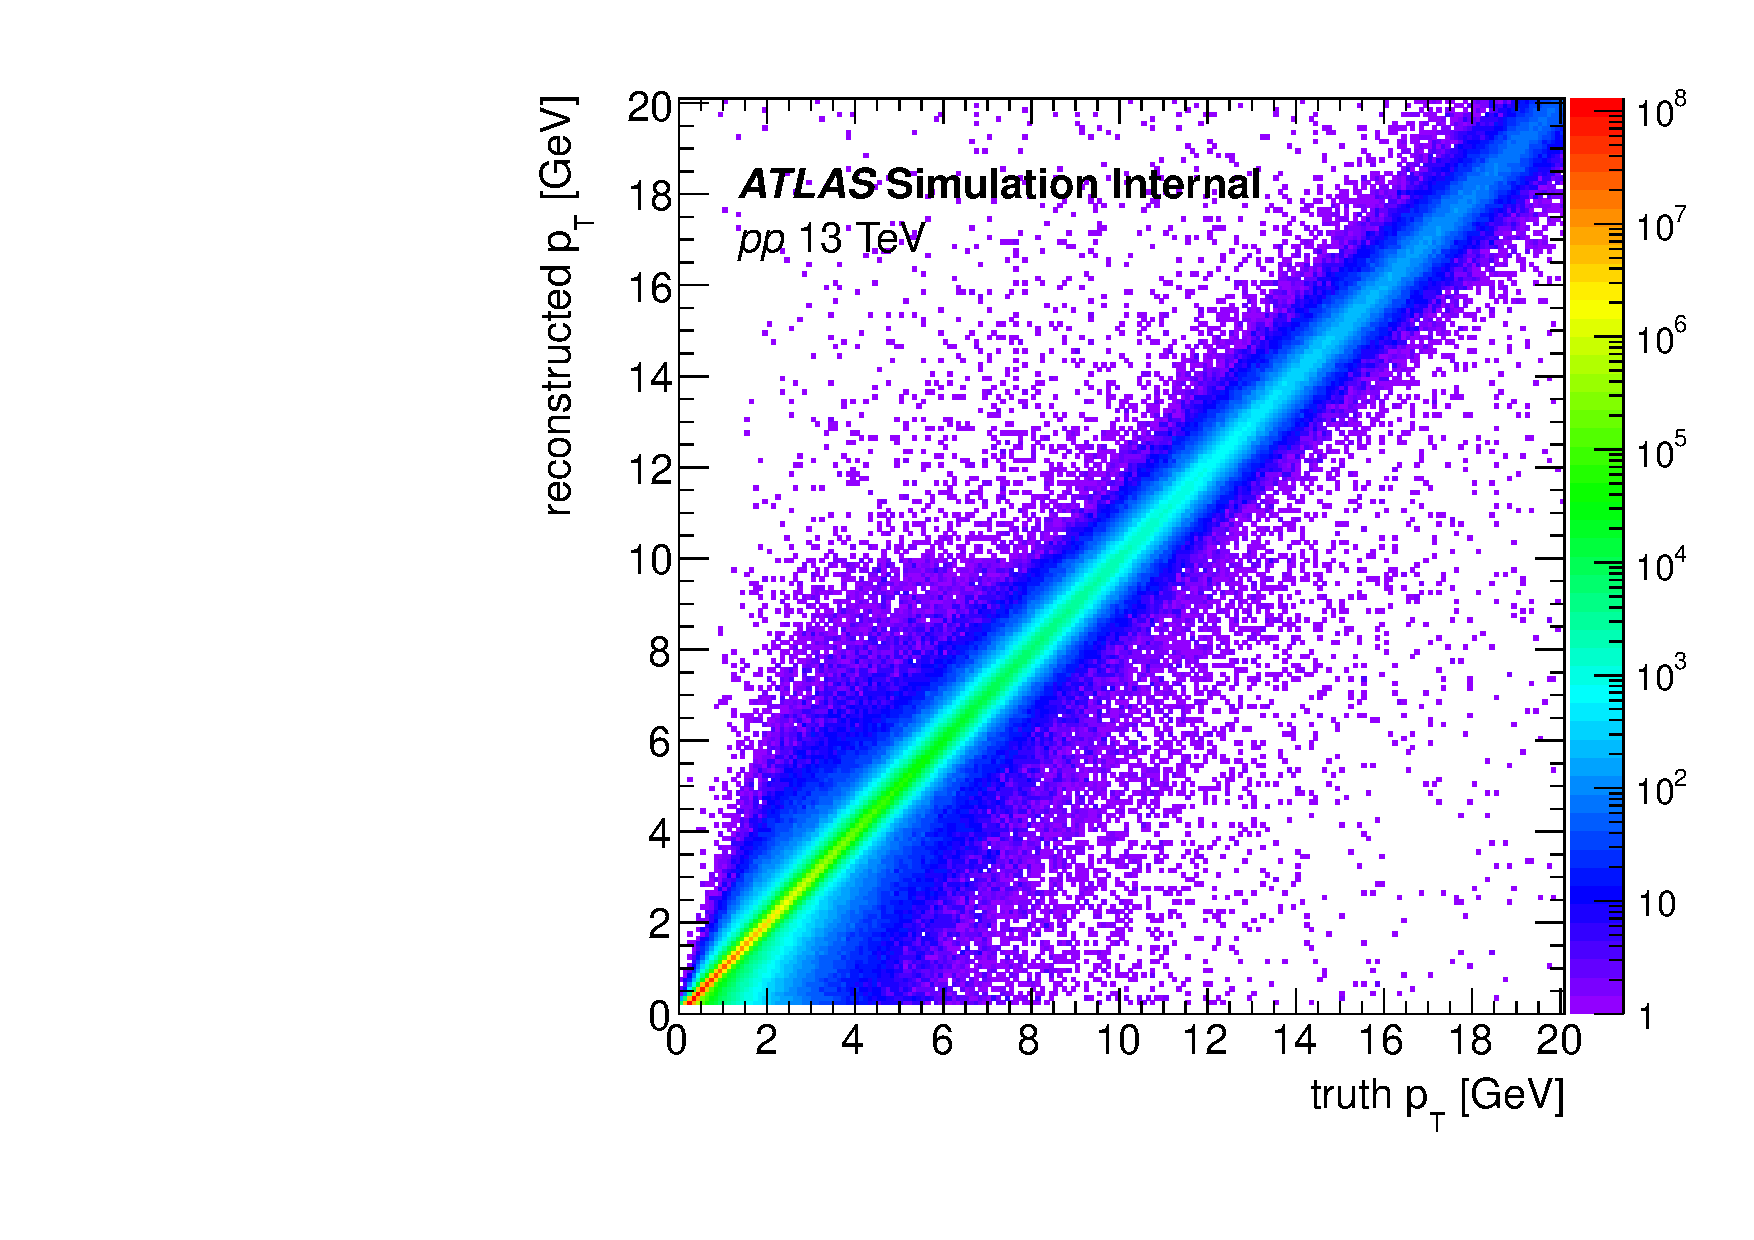
\includegraphics[width=1.\linewidth]{figs/sec_evtSlc/trkEff_pp13_mon_crr_pT.pdf}
\caption{Correlation of truth and reconstructed.}
\end{subfigure}
\begin{subfigure}{0.5\textwidth}
\centering
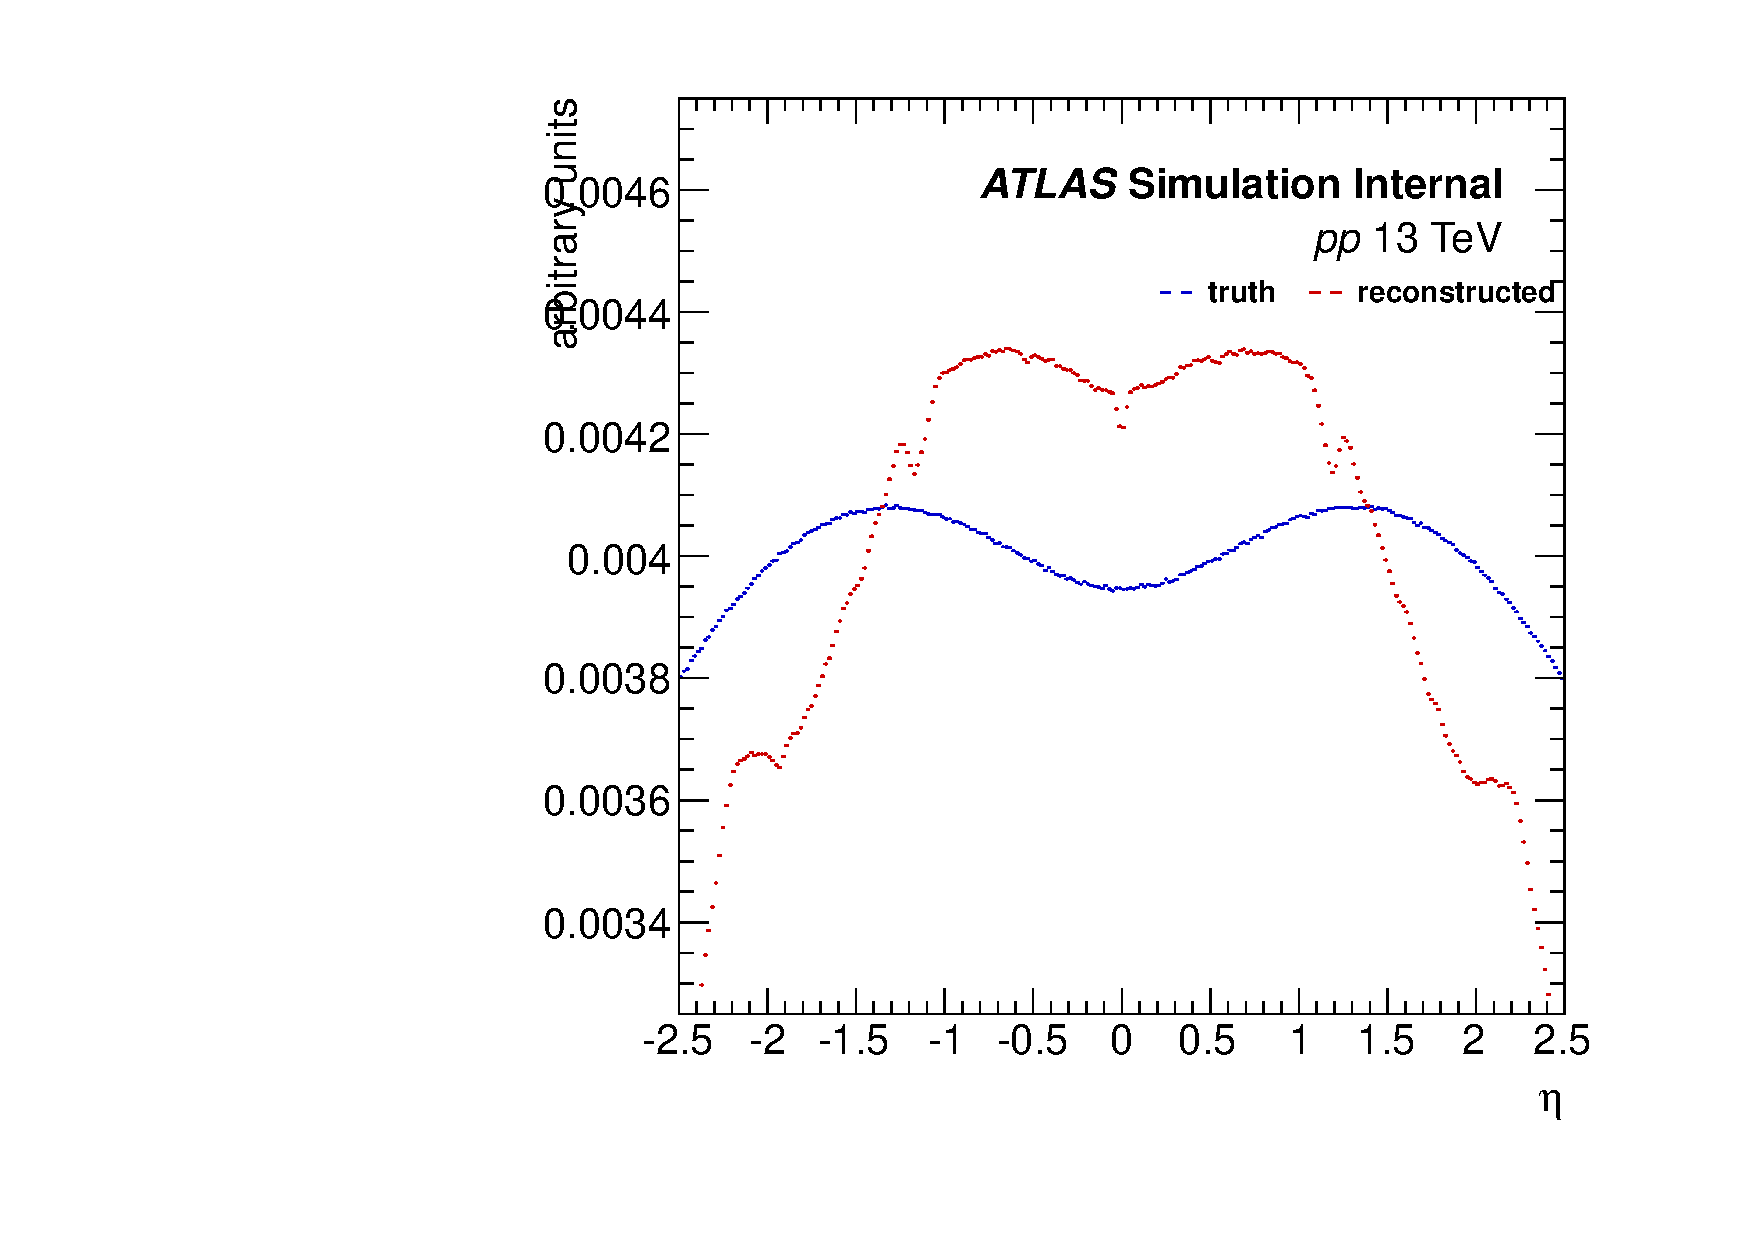
\includegraphics[width=1.\linewidth]{figs/sec_evtSlc/trkEff_pp13_mon_dis_eta.pdf}
\caption{Distribution of $\eta$.}
\end{subfigure}
\begin{subfigure}{0.5\textwidth}
\centering
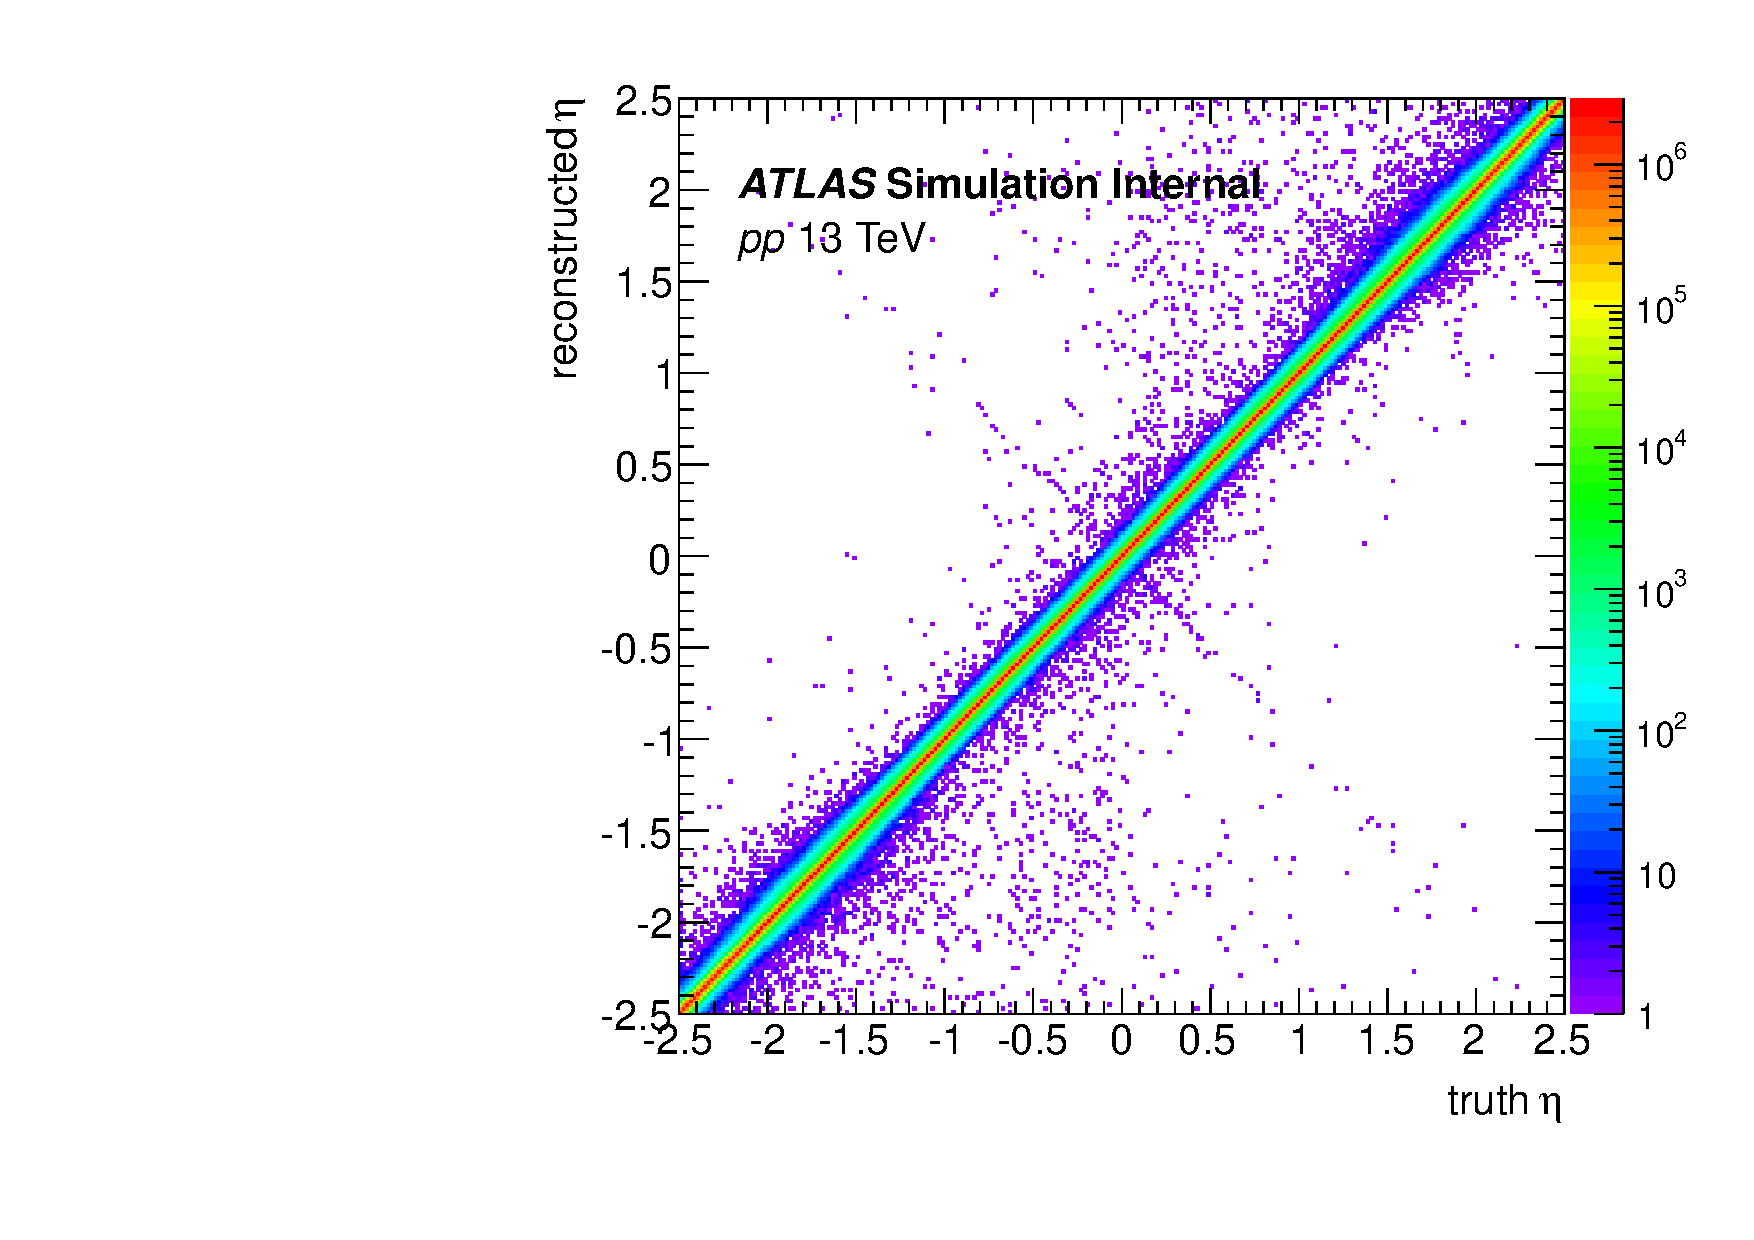
\includegraphics[width=1.\linewidth]{figs/sec_evtSlc/trkEff_pp13_mon_crr_eta.pdf}
\caption{Correlation of truth and reconstructed.}
\end{subfigure}
\begin{subfigure}{0.5\textwidth}
\centering
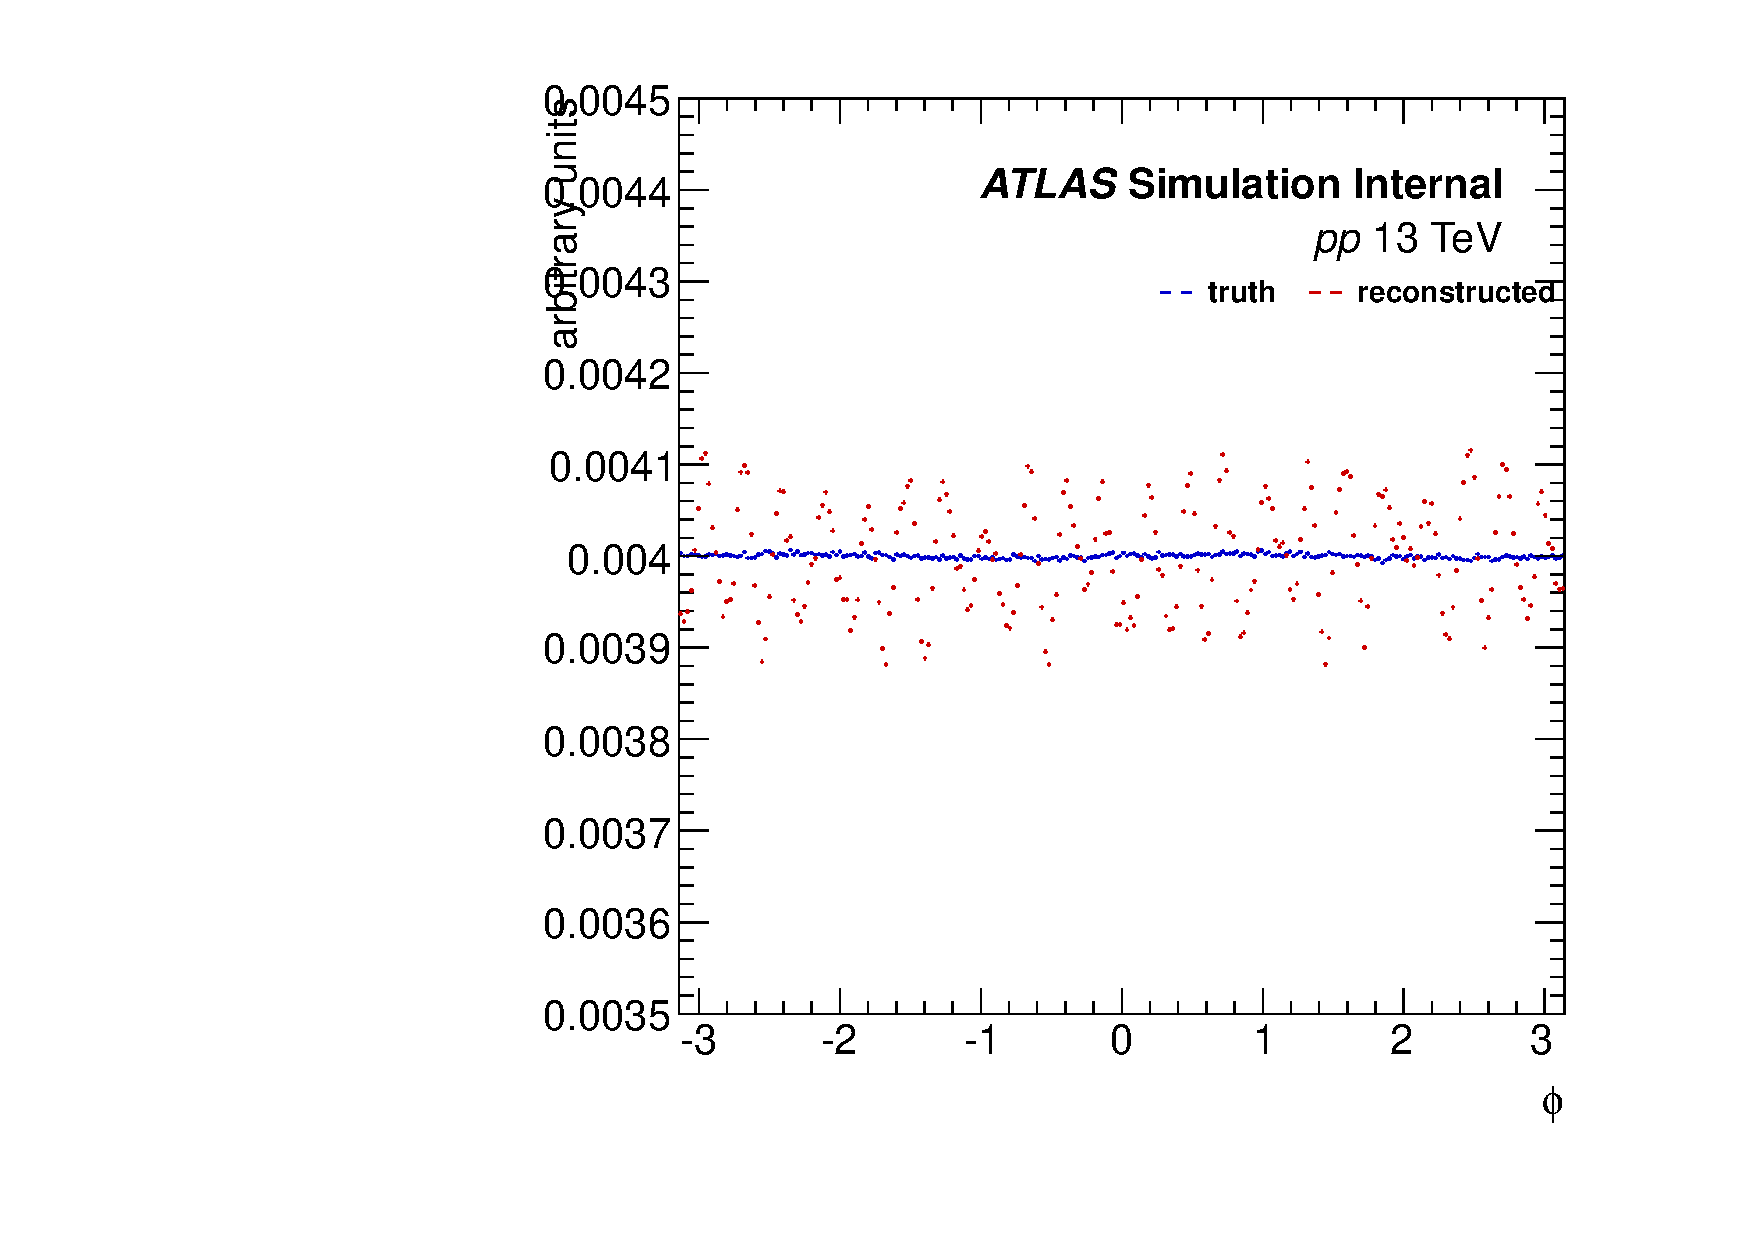
\includegraphics[width=1.\linewidth]{figs/sec_evtSlc/trkEff_pp13_mon_dis_phi.pdf}
\caption{Distribution of $\phi$.}
\end{subfigure}
\begin{subfigure}{0.5\textwidth}
\centering
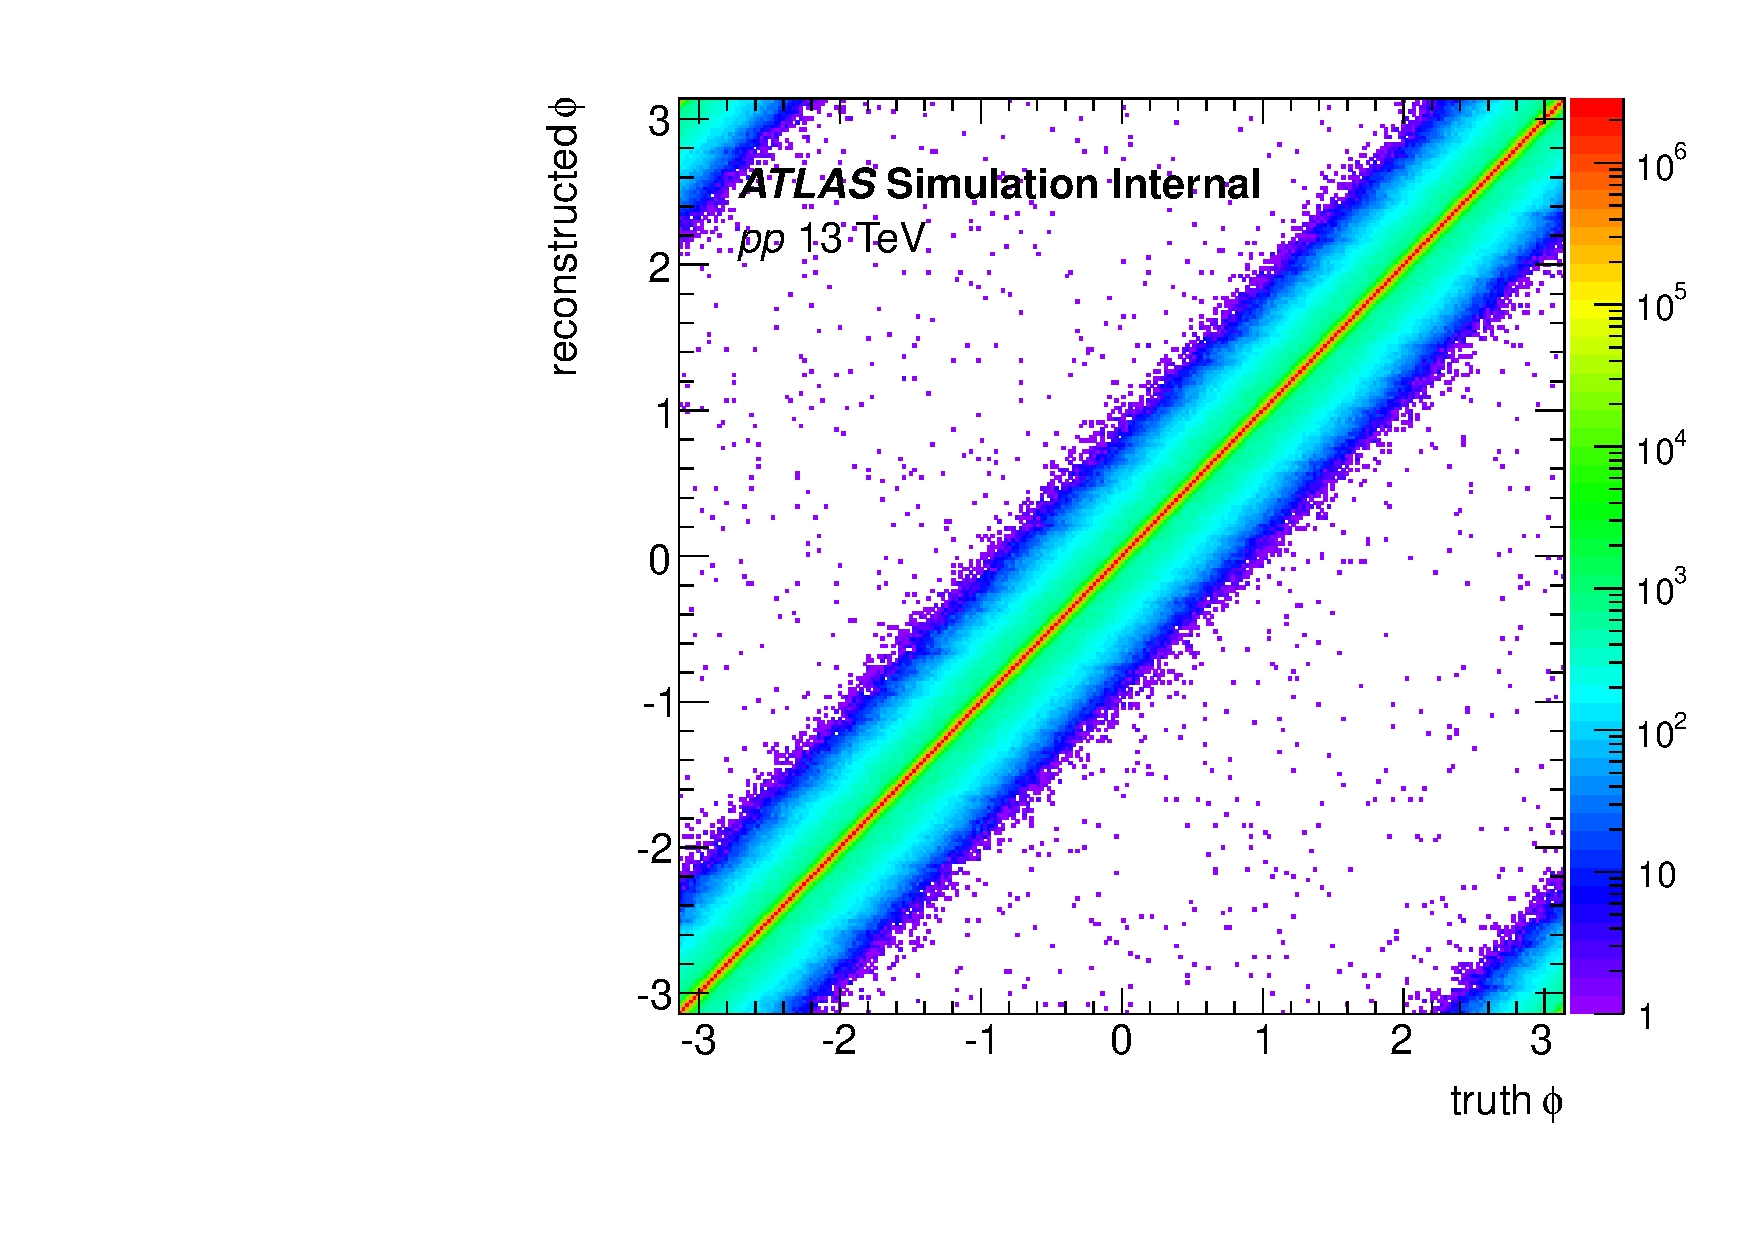
\includegraphics[width=1.\linewidth]{figs/sec_evtSlc/trkEff_pp13_mon_crr_phi.pdf}
\caption{Correlation of truth and reconstructed.}
\end{subfigure}

\caption{Performance of particle-level quantities in PYTHIA 13 TeV $pp$.}
\label{fig:trkEff_pp13_mon_trk}
\end{figure}

In this analysis we also included the PYTHIA truth results as a comparison with data. In order to include more statistics, the min-bias data sets used are on the $\verb|EVGEN|$ level:
\begin{itemize}
\item 200 million non-diffractive events
\begin{itemize}[leftmargin=*]
\item[] \verb|mc15_13TeV.361203.Pythia8_A2_MSTW2008LO_ND_minbias.evgen.EVNT.e3639/|
\end{itemize}
\end{itemize}

\begin{figure}[H]
\centering
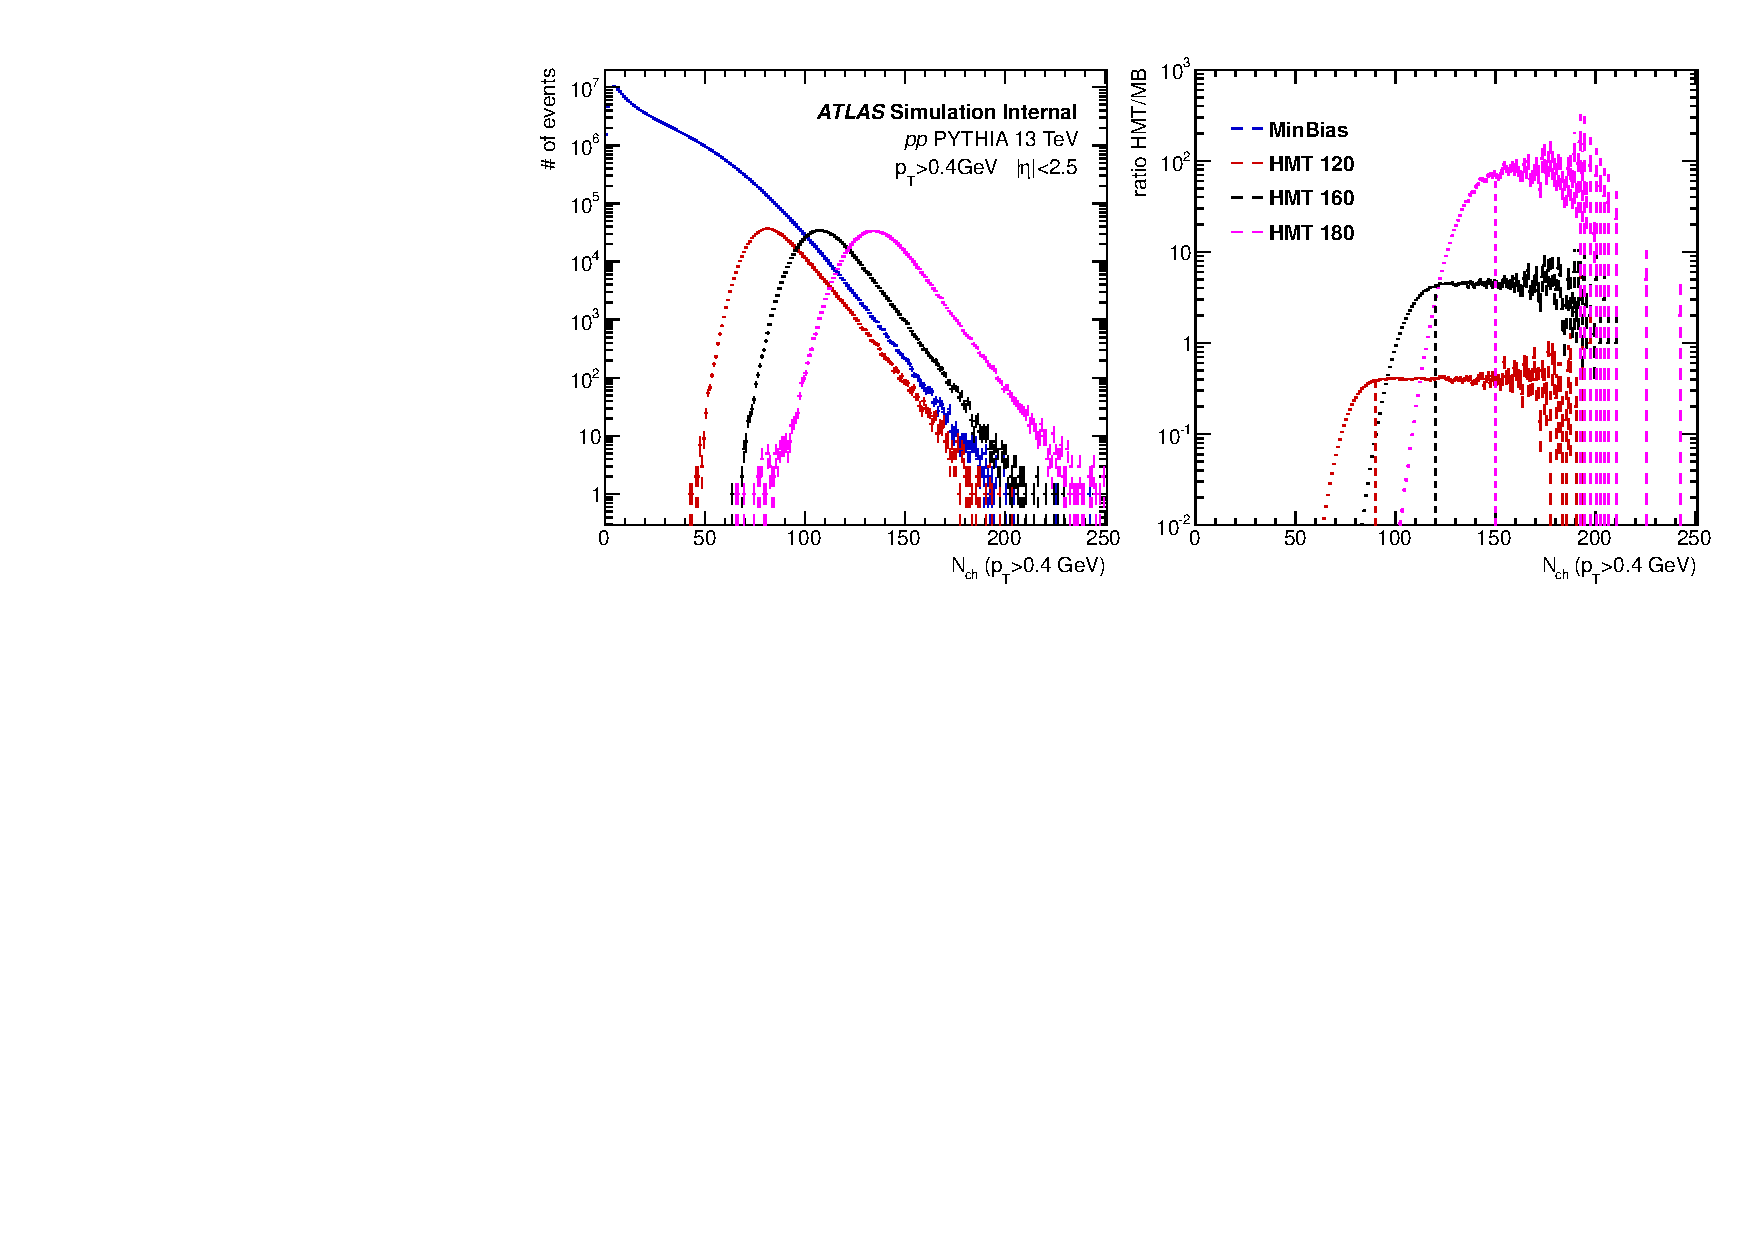
\includegraphics[width=.9\linewidth]{figs/sec_evtSlc/mon_pythia_truth_trkDis.pdf}
\caption{Left plot shows the $N_{ch}$ distribution of MinBias and HMT events separately. Right plot shows the ratio of HMT events and MinBias events. The dash lines in the right plot indicate the minimum $N_{ch}$ cuts while including HMT events, in order to not introduce additional bias.}
\label{fig:mon_pythia_truth_trkDis}
\end{figure}
As to the HMT events, $\verb|EVGEN|$ provides exactly the same statistics as reconstructed sample. In $pp$ data, the high-multiplicity events were selected by using online algorithms, where most of the bias come from the difference between online and offline tracking reconstruction. While in PYTHIA, since it is not clear how the high-multiplicity events are selected, in order not to introduce additional bias, we only select the HMT events where "trigger efficiency" is $100\%$, as indicated in Fig.~\ref{fig:mon_pythia_truth_trkDis}. For three HMT data sets, the $N_{ch}$ cuts are determined as: 90, 120 and 150.



\subsection{Formulas for direct cumulant with particle weight}

\subsubsection{Traditional method}
The idea of direct cumulant is to calculate the multi-particle correlation in a single loop. However, since the multi-particle correlation only counts the unique pairs, some duplicated terms need to be subtracted out.

We start with 2-particle correlation, to calculate $W_{\lr{2}}$:
\begin{equation}
(\sum w_{i})^{2}=\sum w_{i}w_{j}+\sum w_{i}^{2}
\end{equation}
where in the following equations, all summation symbols mean summing the unique pairs for simplicity. We also introduce the notation $S_{p}^{k}$ for better book keeping:
\begin{equation}
S_{p}^{k}\equiv(\sum w_{i}^{p})^{k}
\end{equation}

So the goal of direct cumulant is to express the 2- and 4-particle correlation as a function of $Q_{n},k$ and $S_{p}^{k}$, so that they could be calculated in a single loop.
\begin{equation}
\begin{split}
corr_{n}\{2\}&\to f(Q_{n,k},S_{p}^{k}) \\
corr_{n}\{4\}&\to g(Q_{n,k},S_{p}^{k})
\end{split}
\end{equation}

In the same way, in order to calculate $\sum w_{i}w_{j}e^{\text{i}n(\phi_{i}-\phi_{j})}$, we expand:
\begin{equation}
\begin{split}
(\sum w_{i}e^{in\phi_{i}})^{2}&=\sum w_{i}^{2}+\sum w_{i}w_{j}e^{in(\phi_{i}-\phi_{j})} \\
\Rightarrow |Q_{n,1}|^{2}&=S_{2}^{1}+\sum w_{i}w_{j}e^{\text{i}n(\phi_{i}-\phi_{j})}
\end{split}
\end{equation}
and plug in all the formulas above, we get the expression for $corr_{n}\{2\}$
\begin{equation}
\begin{split}
W_{\lr{2}}&=S_{1}^{2}-S_{2}^{1} \\
corr_{n}\{2\}&=\frac{|Q_{n,1}|^{2}-S_{2}^{1}}{S_{1}^{2}-S_{2}^{1}}
\end{split}
\end{equation}

The formula for 4-particle correlations will be more complicated. We will start with $W_{\lr{4}}$ by expanding $S_{1}^{4}$:
\begin{equation}
S_{1}^{4} = \sum w_{i}w_{j}w_{k}w_{l}+6\sum w_{i}^{2}w_{j}w_{k}+3\sum w_{i}^{2}w_{j}^{2}+4\sum w_{i}^{3}w_{j}+S_{4}^{1}
\end{equation}
where in order to calculate the remaining non-$S$ terms, proper terms also need to be expanded:
\begin{equation}
\begin{split}
S_{3}^{1}S_{1}^{1}&=\sum w_{i}^{3}w_{j}+S_{4}^{1} \\
S_{2}^{2}&=\sum w_{i}^{2}w_{j}^{2}+S_{4}^{1} \\
S_{2}^{1}S_{1}^{2}&=\sum w_{i}^{2}w_{j}w_{k}+2\sum w_{i}^{3}w_{j}+\sum w_{i}^{2}w_{j}^{2}+S_{4}^{1}
\end{split}
\end{equation}

By solving the linear equation, we get:
\begin{equation}
\sum w_{i}w_{j}w_{k}w_{l} = S_{1}^{4}+8S_{3}^{1}S_{1}^{1}-6S_{2}^{1}S_{1}^{2}+3S_{2}^{2}-6S_{4}^{1}
\end{equation}

In order to simply the writing, we define:
\begin{equation}
e^{\text{i}n\phi_{i}}\equiv q_{i}
\end{equation}
where we omitted the harmonic $n$ and we will follow a new approach to derive the $corr_{n}\{4\}$ without tracking weight, which proves its benefits in the case of track efficiency correction:
\begin{equation}
\begin{split}
\sum q_{i}^{}\sum q_{i}^{*}\sum q_{i}^{}\sum q_{i}^{*}&=\sum q_{i}^{}q_{j}^{*}q_{k}^{}q_{l}^{*} \\
&+4\sum q_{i}^{}q_{i}^{*}q_{j}^{}q_{k}^{*}+2\sum q_{i}^{}q_{j}^{*}q_{i}^{}q_{k}^{*} \\
&+2\sum q_{i}^{}q_{i}^{*}q_{j}^{}q_{j}^{*}+\sum q_{i}^{}q_{j}^{*}q_{i}^{}q_{j}^{*} \\
&+4\sum q_{i}^{}q_{i}^{*}q_{i}^{}q_{j}^{*} \\
&+\sum q_{i}^{}q_{i}^{*}q_{i}^{}q_{i}^{*}
\end{split}
\end{equation}
where $q_{i}^{}\equiv Q$ and $q_{i}^{*}\equiv Q^{*}$. Follow the similar way, many terms in above formulas can be further expanded. Like calculating $W_{\lr{4}}$, the goal is to express the final form as a function of $Q$:
\begin{equation}
\begin{split}
\sum q_{i}^{}q_{i}^{*}q_{i}^{} \sum q_{i}^{*} &= \sum q_{i}^{}q_{i}^{*}q_{i}^{}q_{j}^{*} + \sum q_{i}^{}q_{i}^{*}q_{i}^{}q_{i}^{*} \\
\Rightarrow \sum q_{i}^{}q_{i}^{*}q_{i}^{}q_{j}^{*} &= |Q_{n}|^{2}-M \\
& \\
\sum q_{i}^{}q_{i}^{*}\sum q_{i}^{}q_{i}^{*} &= \sum q_{i}^{}q_{i}^{*}q_{j}^{}q_{j}^{*} + \sum q_{i}^{}q_{i}^{*}q_{i}^{}q_{i}^{*} \\
\Rightarrow \sum q_{i}^{}q_{i}^{*}q_{j}^{}q_{j}^{*} &= M^{2}-M \\
& \\
\sum q_{i}^{}q_{i}^{} \sum q_{i}^{*}q_{i}^{*} &= \sum q_{i}^{}q_{j}^{*}q_{i}^{}q_{j}^{*} + \sum q_{i}^{}q_{i}^{*}q_{i}^{}q_{i}^{*} \\
\Rightarrow \sum q_{i}^{}q_{j}^{*}q_{i}^{}q_{j}^{*} &= |Q_{2n}|^{2}-M \\
& \\
\sum q_{i}^{}q_{i}^{*} \sum q_{i}^{} \sum q_{i}^{*} &= \sum q_{i}^{}q_{i}^{*}q_{j}^{}q_{k}^{*} + 2 \sum q_{i}^{}q_{i}^{*}q_{i}^{}q_{j}^{*} + \sum q_{i}^{}q_{i}^{*}q_{j}^{}q_{j}^{*} + \sum q_{i}^{}q_{i}^{*}q_{i}^{}q_{i}^{*} \\
\Rightarrow \sum q_{i}^{}q_{i}^{*}q_{j}^{}q_{k}^{*} &= (M-2)|Q_{n}|^{2}-M^{2}+2M \\
& \\
\sum q_{i}^{}q_{i}^{}\sum q_{i}^{*}\sum q_{i}^{*} &= \sum q_{i}^{}q_{j}^{*}q_{i}^{}q_{k}^{*} + 2\sum q_{i}^{}q_{i}^{*}q_{i}^{}q_{j}^{*} + \sum q_{i}^{}q_{j}^{*}q_{i}^{}q_{j}^{*} + \sum q_{i}^{}q_{i}^{*}q_{i}^{}q_{i}^{*} \\
\Rightarrow \sum q_{i}^{}q_{j}^{*}q_{i}^{}q_{k}^{*} &= |Q_{2n}^{}Q_{n}^{*}Q_{n}^{*}|-|Q_{2n}|^{2}-2|Q_{n}|^{2}+2M
\end{split}
\end{equation}

By solving the linear equations above, we could get:
\begin{equation}
\sum q_{i}^{}q_{j}^{*}q_{k}^{}q_{l}^{*} = |Q_{n}|^{4}+|Q_{2n}|^{2}-2|Q_{2n}^{}Q_{n}^{*}Q_{n}^{*}|-4(M-2)|Q_{n}|^{2}+2M(M-3)
\end{equation}
where the result is identical to the procedure described in the direct cumulant paper.

The advantage of this approach is to deal with track weights. $q_{i}$ is then modified as:
\begin{equation}
w_{i}e^{\text{i}n\phi_i}\equiv q_{i}
\end{equation}
and then all the expansions can be easily obtained by slightly modifying some of the summation terms:
\begin{equation}
\begin{split}
\sum q_{i}^{}q_{i}^{*}q_{i}^{} \sum q_{i}^{*} &= \sum q_{i}^{}q_{i}^{*}q_{i}^{}q_{j}^{*} + \sum q_{i}^{}q_{i}^{*}q_{i}^{}q_{i}^{*} \\
\Rightarrow \sum q_{i}^{}q_{i}^{*}q_{i}^{}q_{j}^{*} &= |Q_{n,3}^{}Q_{n,1}^{*}|-S_{4}^{1} \\
& \\
\sum q_{i}^{}q_{i}^{*}\sum q_{i}^{}q_{i}^{*} &= \sum q_{i}^{}q_{i}^{*}q_{j}^{}q_{j}^{*} + \sum q_{i}^{}q_{i}^{*}q_{i}^{}q_{i}^{*} \\
\Rightarrow \sum q_{i}^{}q_{i}^{*}q_{j}^{}q_{j}^{*} &= S_{2}^{2}-S_{4}^{1} \\
& \\
\sum q_{i}^{}q_{i}^{} \sum q_{i}^{*}q_{i}^{*} &= \sum q_{i}^{}q_{j}^{*}q_{i}^{}q_{j}^{*} + \sum q_{i}^{}q_{i}^{*}q_{i}^{}q_{i}^{*} \\
\Rightarrow \sum q_{i}^{}q_{j}^{*}q_{i}^{}q_{j}^{*} &= |Q_{2n,2}|^{2}-S_{4}^{1} \\
& \\
\sum q_{i}^{}q_{i}^{*} \sum q_{i}^{} \sum q_{i}^{*} &= \sum q_{i}^{}q_{i}^{*}q_{j}^{}q_{k}^{*} + 2 \sum q_{i}^{}q_{i}^{*}q_{i}^{}q_{j}^{*} + \sum q_{i}^{}q_{i}^{*}q_{j}^{}q_{j}^{*} + \sum q_{i}^{}q_{i}^{*}q_{i}^{}q_{i}^{*} \\
\Rightarrow \sum q_{i}^{}q_{i}^{*}q_{j}^{}q_{k}^{*} &= S_{2}^{1}|Q_{n,1}|^{2}-2|Q_{n,3}^{}Q_{n,1}^{*}|-S_{2}^{2}+2S_{4}^{1} \\
& \\
\sum q_{i}^{}q_{i}^{}\sum q_{i}^{*}\sum q_{i}^{*} &= \sum q_{i}^{}q_{j}^{*}q_{i}^{}q_{k}^{*} + 2\sum q_{i}^{}q_{i}^{*}q_{i}^{}q_{j}^{*} + \sum q_{i}^{}q_{j}^{*}q_{i}^{}q_{j}^{*} + \sum q_{i}^{}q_{i}^{*}q_{i}^{}q_{i}^{*} \\
\Rightarrow \sum q_{i}^{}q_{j}^{*}q_{i}^{}q_{k}^{*} &= |Q_{2n,2}^{}Q_{n,1}^{*}Q_{n,1}^{*}|-|Q_{2n,2}|^{2}-2|Q_{n,3}^{}Q_{n,1}^{*}|+2S_{4}^{1}
\end{split}
\end{equation}

By solving the linear equations above, we could get:
\begin{equation}
\sum q_{i}^{}q_{j}^{*}q_{k}^{}q_{l}^{*} = |Q_{n,1}|^{4}+|Q_{2n,2}|^{2}-2|Q_{2n,2}^{}Q_{n,1}^{*}Q_{n,1}^{*}|+8|Q_{n,3}^{}Q_{n,1}|-4S_{2}^{1}|Q_{n,1}|^{2}+2S_{2}^{2}-6S_{4}^{1}
\end{equation}
and the result is consistent with original direct cumulant paper.

\subsubsection{2 sub-event method: $1st$ kind}
The formulas for 2 sub-event method will be simpler compared with traditional cumulant, because some duplicated terms no longer show up. For the purpose of better book keeping, we will define the new $Q_{n,k}$ and $S_{p}^{k}$ for the sub-event case. In the following formulas, subscript $i$ and $j$ denote particles from sub-event $A$ and subscript $k$ and $l$ denote particles from sub-event $B$:
\begin{equation}
\begin{split}
A_{n,k}&\equiv \sum w_{i}^{k}e^{\text{i}n\phi_{i}} \\
B_{n,k}&\equiv \sum w_{l}^{k}e^{\text{i}n\phi_{l}}
\end{split}
\end{equation}
\begin{equation}
\begin{split}
X_{p}^{k}&\equiv (\sum w_{i}^{p})^{k} \\
Y_{p}^{k}&\equiv (\sum w_{l}^{p})^{k} \\
\end{split}
\end{equation}

The expression for $W_{\lr{2_{a|b}}}$ is much simpler since two particles come from two sub-events and they can never be the same particle:
\begin{equation}
W_{\lr{2_{a|b}}}\equiv \sum w_{i}w_{k} = \sum w_{i} \sum w_{j} = X_{1}^{1}Y_{1}^{1}
\end{equation}
In a similar way, $W_{\lr{4_{a,a|b,b}}}$ can also be determined:
\begin{equation}
W_{\lr{4_{a,a|b,b}}} = X_{1}^{2}Y_{1}^{2}-X_{2}^{1}Y_{1}^{2}-X_{1}^{2}Y_{2}^{1}+X_{2}^{1}Y_{2}^{1}
\end{equation}

For the $1st$ kind of 2 sub-event method, two particles from the same sub-event always have the same sign. We still use the same notation $q_{i}$ as the traditional cumulant method, only the subscript determines which sub-event it comes from: $i,j$ from one sub-event and $k,l$ from the other sub-event:
\begin{equation}
\sum q_{i}^{} \sum q_{k}^{*} = \sum q_{i}^{}q_{k}^{*}
\end{equation}
and for 4-particle cumulant:
\begin{equation}
\begin{split}
\sum q_{i}^{} \sum q_{i}^{} \sum q_{k}^{*} \sum q_{k}^{*} &= \sum q_{i}^{}q_{j}^{}q_{k}^{*}q_{l}^{*} + \sum q_{i}^{}q_{i}^{}q_{k}^{*}q_{l}^{*} + \sum q_{i}^{}q_{j}^{}q_{k}^{*}q_{k}^{*} + \sum q_{i}^{}q_{i}^{}q_{k}^{*}q_{k}^{*} \\
\sum q_{i}^{}q_{i}^{} \sum q_{k}^{*}q_{k}^{*} &= \sum q_{i}^{}q_{i}^{} \sum q_{k}^{*}q_{k}^{*} \\
\sum q_{i}^{}q_{i}^{} \sum q_{k}^{*} \sum q_{k}^{*} &= \sum q_{i}^{}q_{i}^{}q_{k}^{*}q_{l}^{*} + \sum q_{i}^{}q_{i}^{}q_{k}^{*}q_{k}^{*} \\
\sum q_{i}^{} \sum q_{i}^{} \sum q_{k}^{*}q_{k}^{*} &= \sum q_{i}^{}q_{j}^{}q_{k}^{*}q_{k}^{*} + \sum q_{i}^{}q_{i}^{}q_{k}^{*}q_{k}^{*}
\end{split}
\end{equation}

Solve the linear equations and plug in $A_{n,k}$ and $B_{n,k}$:
\begin{equation}
\sum q_{i}^{}q_{j}^{}q_{k}^{*}q_{l}^{*} = |A_{n,1}^{}B_{n,1}^{*}A_{n,1}^{}B_{n,1}^{*}|-|A_{2n,2}^{}B_{n,1}^{*}B_{n,1}^{*}|-|A_{n,1}^{}A_{n,1}^{}B_{2n,2}^{*}|+|A_{2n,2}^{}B_{2n,2}^{*}|
\end{equation}
where $'|  |'$ means taking the real part of the inner product.

\subsubsection{2 sub-event method: $2nd$ kind}
Keeping all the same notations from $1st$ kind, here we list all the formulas for the 2 sub-event $2nd$ kind.
For $W_{\lr{2}}$, there are three items:
\begin{equation}
\begin{split}
W_{\lr{2_{a|a}}} &\equiv \sum w_{i}w_{j} = \sum w_{i} \sum w_{i} - \sum w_{i}^{2} \\
W_{\lr{2_{b|b}}} &\equiv \sum w_{k}w_{l} = \sum w_{k} \sum w_{k} - \sum w_{k}^{2} \\
W_{\lr{2_{a|b}}} &\equiv \sum w_{i}w_{k} = \sum w_{i} \sum w_{k}
\end{split}
\end{equation}
and expression for $W_{\lr{4_{a,b|a,b}}}$ is same as $1st$ kind because conjugate will not change the track weight, which is a real number:
\begin{equation}
W_{\lr{4_{a,b|a,b}}} = X_{1}^{2}Y_{1}^{2}-X_{2}^{1}Y_{1}^{2}-X_{1}^{2}Y_{2}^{1}+X_{2}^{1}Y_{2}^{1}
\end{equation}

Compared with $1st$ kind, the expression for $\sum q_{i}^{}q_{j}^{*}q_{k}^{}q_{l}^{*}$ is similar:
\begin{equation}
\begin{split}
\sum q_{i}^{} \sum q_{i}^{*} \sum q_{k}^{} \sum q_{k}^{*} &= \sum q_{i}^{}q_{j}^{*}q_{k}^{}q_{l}^{*} + \sum q_{i}^{}q_{i}^{*}q_{k}^{}q_{l}^{*} + \sum q_{i}^{}q_{j}^{*}q_{k}^{}q_{k}^{*} + \sum q_{i}^{}q_{i}^{*}q_{k}^{}q_{k}^{*} \\
\sum q_{i}^{}q_{i}^{*} \sum q_{k}^{}q_{k}^{*} &= \sum q_{i}^{}q_{i}^{*} \sum q_{k}^{}q_{k}^{*} \\
\sum q_{i}^{}q_{i}^{*} \sum q_{k}^{} \sum q_{k}^{*} &= \sum q_{i}^{}q_{i}^{*}q_{k}^{}q_{l}^{*} + \sum q_{i}^{}q_{i}^{*}q_{k}^{}q_{k}^{*} \\
\sum q_{i}^{} \sum q_{i}^{*} \sum q_{k}^{}q_{k}^{*} &= \sum q_{i}^{}q_{j}^{*}q_{k}^{}q_{k}^{*} + \sum q_{i}^{}q_{i}^{*}q_{k}^{}q_{k}^{*}
\end{split}
\end{equation}
and the 4-particle correlation:
\begin{equation}
\sum q_{i}^{}q_{j}^{*}q_{k}^{}q_{l}^{*} = |A_{n,1}^{}A_{n,1}^{*}B_{n,1}^{}B_{n,1}^{*}|-X_{2}^{1}|B_{n,1}|^{2}-Y_{2}^{1}|A_{n,1}|^{2}+X_{2}^{1}Y_{2}^{1}
\end{equation}

\subsubsection{3 sub-event method: $1st$ kind}
Since there is one more sub-event, we will change our notations as:
\begin{equation}
\begin{split}
A_{n,k}&\equiv \sum w_{i}^{k}e^{\text{i}n\phi_{i}} \\
B_{n,k}&\equiv \sum w_{k}^{k}e^{\text{i}n\phi_{k}} \\
C_{n,k}&\equiv \sum w_{l}^{k}e^{\text{i}n\phi_{l}}
\end{split}
\end{equation}
\begin{equation}
\begin{split}
X_{p}^{k}&\equiv (\sum w_{i}^{p})^{k} \\
Y_{p}^{k}&\equiv (\sum w_{k}^{p})^{k} \\
Z_{p}^{k}&\equiv (\sum w_{l}^{p})^{k}
\end{split}
\end{equation}
where in the following formulas 2 of 4 particles always come from sub-event $A$, denoted as subscript $i$ and $j$. Particle $k$ comes from sub-event $B$ and particle $l$ comes from sub-event $C$. All the other permutations can be easily obtained by rotating the $A,B$ and $C$.

All the formulas can be directly "guessed" from without weights case and they are summarized below:
\begin{equation}
\begin{split}
W_{\lr{2_{a|b}}} &= X_{1}^{1}Y_{1}^{1} \\
W_{\lr{2_{a|c}}} &= X_{1}^{1}Z_{1}^{1} \\
W_{\lr{4_{a,a|b,c}}} &= (X_{1}^{2}-X_{2}^{1})Y_{1}^{1}Z_{1}^{1} \\
\sum q_{i}^{}q_{k}^{*} &= |A_{n,1}B_{n,1}^{*}| \\
\sum q_{i}^{}q_{l}^{*} &= |A_{n,1}C_{n,1}^{*}| \\
\sum q_{i}^{}q_{j}^{*}q_{k}^{}q_{l}^{*} &= |A_{n,1}^{}B_{n,1}^{*}A_{n,1}^{}C_{n,1}^{*}|-|A_{2n,2}^{}B_{n,1}^{*}C_{n,1}^{*}|
\end{split}
\end{equation}

\subsubsection{3 sub-event method: $2nd$ kind}
Use same notation as the $1st$ kind, all the formulas are listed below:
\begin{equation}
\begin{split}
W_{\lr{2_{a|b}}} &= X_{1}^{1}Y_{1}^{1} \\
W_{\lr{2_{a|c}}} &= X_{1}^{1}Z_{1}^{1} \\
W_{\lr{2_{b|c}}} &= Y_{1}^{1}Z_{1}^{1} \\
W_{\lr{2_{a|a}}} &= X_{1}^{2}-X_{2}^{1} \\
W_{\lr{4_{a,b|a,c}}} &= (X_{1}^{2}-X_{2}^{1})Y_{1}^{1}Z_{1}^{1} \\
\sum q_{i}^{}q_{k}^{*} &= |A_{n,1}B_{n,1}^{*}| \\
\sum q_{i}^{}q_{l}^{*} &= |A_{n,1}C_{n,1}^{*}| \\
\sum q_{k}^{}q_{l}^{*} &= |B_{n,1}C_{n,1}^{*}| \\
\sum q_{i}^{}q_{j}^{*} &= |A_{n,1}|^{2}-X_{2}^{1} \\
\sum q_{i}^{}q_{j}^{*}q_{k}^{}q_{l}^{*} &= |A_{n,1}^{}A_{n,1}^{*}B_{n,1}^{}C_{n,1}^{*}|-X_{2}^{1}|B_{n,1}^{*}C_{n,1}^{*}|
\end{split}
\end{equation}



